\documentclass{article}

%% Language and font encodings
\usepackage[english]{babel}
\usepackage[utf8x]{inputenc}
\usepackage[T1]{fontenc}
\usepackage{amsfonts}
\usepackage[margin=41mm]{geometry}

%% Sets page size and margins
%\usepackage[a4paper,top=3cm,bottom=2cm,left=3cm,right=3cm,marginparwidth=1.75cm]{geometry}

%% Useful packages
\usepackage[colorlinks=true, allcolors=black]{hyperref}
\usepackage{amsmath}
\usepackage{xcolor}
\usepackage{amssymb}
\usepackage{amsthm}
\usepackage{stmaryrd}
\usepackage{graphicx}
\usepackage{enumitem}
\usepackage{tikz, pgfplots}
\usetikzlibrary{positioning}

%Theorem
\theoremstyle{plain}
\newtheorem{theorem}{Theorem}[subsection]
\newtheorem{proposition}[theorem]{Proposition}
\newtheorem{lemma}[theorem]{Lemma}
\newtheorem*{corollary}{Corollary}
\theoremstyle{definition}
\newtheorem*{definition}{Definition}

%Usual Sets
\newcommand{\C}{\mathbb{C}}
\newcommand{\R}{\mathbb{R}}
\newcommand{\Q}{\mathbb{Q}}
\newcommand{\Z}{\mathbb{Z}}
\newcommand{\N}{\mathbb{N}}
\newcommand{\F}{\mathbb{F}}
\newcommand{\E}{\mathbb{E}}
\newcommand{\K}{\mathbb{K}}
\newcommand{\Zn}[1]{\mathbb{Z}/ #1 \mathbb{Z}}

%Special Sets
\newcommand{\Iint}[2]{\llbracket #1 , #2 \rrbracket}

%Math Operators
\let\Re\relax
\let\Im\relax
\DeclareMathOperator{\Im}{Im}
\DeclareMathOperator{\Re}{Re}
\DeclareMathOperator{\Null}{null}
\DeclareMathOperator{\range}{range}
\DeclareMathOperator{\card}{card}
\DeclareMathOperator{\Aut}{Aut}
\DeclareMathOperator{\Hom}{Hom}
\DeclareMathOperator{\Gal}{Gal}
\DeclareMathOperator{\Char}{char}

%Others
\newcommand{\td}{\textcolor{red}{\textbf{TODO}}}
\newcommand{\isomorphic}{\cong}

%Example environment
\newenvironment{example}{\noindent\textbf{Example:} \vspace{-0.2cm}\begin{itemize}}{\end{itemize}}

%Remark environment
\newenvironment{remark}{\noindent\textbf{Remark:}}{}

%Notation environment
\newenvironment{notation}{\noindent\textit{Notation:}}{}

%Terminology environment
\newenvironment{terminology}{\noindent\textit{Terminology:}}{}

%Set QED symbol to blacksquare
\renewcommand\qedsymbol{$\blacksquare$}

%Start at section 0
\setcounter{section}{-1}


\title{MATH 457 Notes : Galois Theory}
\author{Samy Lahlou}
\date{}

\begin{document}

\maketitle

These notes are based on lectures given by Professor Henri Darmon at McGill University in Winter 2025. The subject of these lectures is Representation Theory and Galois Theory but I chose to only take notes for the Galois Theory part. \\
As a disclaimer, it is more than possible that I made some mistakes. Feel free to correct me or ask me anything about the content of this document at the following address : samy.lahloukamal@mcgill.ca

\tableofcontents

\newpage

\section{Preliminaries: Fields and Polynomials}

This section is not part of the given lectures but I chose to include it in my notes. The goal is to make an inventory of the non-obvious results used later that would break the rythm if explained in the middle of the following sections.

\subsection{Finite Fields}

The two main mathematical objects studied in Galois Theory are fields, that we will mostly denote by $\F$, $\E$ or sometimes $\K$, and their corresponding ring of polynomials, $\F[x]$, $\E[x]$ and $\K[x]$ respectively. This subsection will be focused on finite fields and their unexpected properties. Most of the following properties are far from being obvious given the definition of a field. 

\begin{definition}
    Given a field $\F$, we denote by $\Char \F$ the least positive integer $n$ such that
    $$\underbrace{1 + 1 + \dots + 1 + 1}_n = 0$$
    and call it the characteristic of $\F$. It there is no such $n$, we write $\Char \F = 0$ and say that $\F$ is a field of characteristic 0.
\end{definition}

If we replace fields with rings in the definition of the characteristic, we know by our experience that there exist rings of any characteristic. More precisely, given a positive integer $n$, we have that $\Zn{n}$ is a ring of characteristic $n$. This turns out to not be the case for fields.

\begin{theorem}
\label{characteristic prime}
    The characteristic of a field is either a prime number or 0.
\end{theorem}

\begin{proof}
    Let $\F$ be a field and suppose that its characteristic is not 0. Define $n = \Char \F$ and suppose that $n$ is a composite number, then there exist positive integers $s$ and $t$ strictly smaller than $n$ such that $n = st$. Define $S$ and $T$ in $\F$ by
    $$S = \underbrace{1 + 1 + \dots + 1 + 1}_s \quad \text{ and } \quad T = \underbrace{1 + 1 + \dots + 1 + 1}_t.$$
    By minimality of $n$, both $S$ and $T$ are non-zero. However, we can show by induction that $S$ and $T$ satisfy
    $$ST = \underbrace{1 + 1 + \dots + 1 + 1}_n = 0$$
    which is in contradiction with the fact that $S$ and $T$ are both non-zero. Therefore, $n$ cannot be composite, and hence, is a prime number.
\end{proof}

From this theorem, we can now understand more precisely the general structure of finite fields. This becomes clearer with the following result.

\begin{corollary}
\label{cardinality finite field power of a prime}
    The cardinality of a finite field is always the power of a prime number.
\end{corollary}

\begin{proof}
    Let $\F$ be a finite field, then its characteristic must be finite since otherwise, $1, 1+1, 1+1+1, ...$ would be an infinite sequence of distinct elements in $\F$. By the previous theorem, there exists a prime number $p$ such that $\Char \F = p$. Consider the ring homomorphism $\varphi : \Z \to \F$ generated by $\varphi(1) = 1$, then in general,
    $$\varphi(n) = \underbrace{1 + 1 + \dots + 1 + 1}_n.$$
    Since $\Char \F = p$, then the kernel of $\varphi$ is $p\Z$. Hence, by the Isomorphism Theorem for ring homomorphisms, the image of $\varphi$ is isomorphic to $\Zn{p}$. Equivalently, $\F$ contains a copy of $\Zn{p}$. Therefore, $\F$ can be viewed as a $\Zn{p}$-vector space since it is closed under scalar multiplication by elements in $\Zn{p}$. Since $\F$ is finite, then it must be a finite-dimensional vector space which means that $\F$ is isomorphic to $(\Zn{p})^n$ as vector spaces for some natural number $n$. It follows that $\# \F = p^n$.
\end{proof}

It turns out the converse is also true: there exists a field of cardinality $p^n$ for all prime number $p$ and natural number $n$. Moreover, any two fields of cardinality $p^n$ are isomorphic. This lets us characterize precisely the finite fields. However, the complete proof of this characterization requires tools that will be introduced in Section \ref{splitting_fields} on Splitting Fields.

One last property of finite fields concerns the structure of their multiplicative group. The following result will be used in the proof of the Primitive Element Theorem in Section \ref{galois_correspondence}.

\begin{theorem}
\label{multiplicative group is cyclic}
    Let $\F$ be a finite field, then $\F^{\times}$ is a cyclic group.
\end{theorem}

\begin{proof}
    Since $\F^{\times}$ is a finite abelian group, then we can apply the Fundamental Theorem of Finitely Generated Abelian Groups to obtain that
    $$\F^{\times} \isomorphic \Z^{d_1} \times \dots \times \Z^{d_t}$$
    where $d_i$ divides $d_{i+1}$ for all $i \in \Iint{1}{t-1}$. It follows that $\F^{\times}$ contains an element of order $d_t$ (take $(0,0, ..., 0, 1)$) and every element has an order that divides $d_t$. Thus, $\alpha^{d_1} = 1$ for all $\alpha \in \F^{\times}$. Consider the polynomial $p(x) = x^{d_t} - 1 \in \F[x]$, notice that it has at most $\deg p = d_t$ roots and that it all the elements of $\F^{\times}$ are roots so $\# \F^{\times} \leq d_t$. Moreover, since $\F^{\times}$ contains an element of order $d_t$, then it has a subgroup of cardinality $d_t$ which shows that $d_t \leq \# \F^{\times}$. Thus, combining the two previous inequalities, $\F^{\times}$ is a group of cardinality $d_t$ which contains an element of order $d_t$, it follows that $\F^{\times}$ is cyclic.
\end{proof}

\subsection{Polynomials over Fields}

Polynomials are at the heart of Galois Theory because of their numerous properties and their complicated structure. A very useful and well known property of polynomials is how similar their behavior is to the integers. This can be illustrated by the following result. 

\begin{theorem}[Euclidean Division]
\label{Euclidean Division}
    Given a field $\F$ and polynomials $f,g \in \F[x]$, there exist unique polynomials $q,r \in \F[x]$ such that
    $$f = qg + r$$
    with $\deg(r) < \deg(g)$.
\end{theorem}

\begin{proof}
    Consider the set
    $$S = \{f-qg : q \in \F[x]\}$$
    and let $r$ be a polynomial in $S$ with minimum degree, then there exists a $q_0 \in \F[x]$ such that
    $f = q_0g + r$. Suppose that $\deg r \geq \deg g$ and write
    $$r(x) = a_n x^n + ... + a_0, \qquad g(x) = b_m x^m + ... + b_0,$$
    with $a_n$ and $b_m$ different than 0, then we obtain that $r_0(x) = r(x) - a_nb_m^{-1}x^{n-m}g(x)$ is a polynomial of degree strictly smaller than $r$ since the terms of higher degree cancel out in the definition of $r_0$. It follows that
    \begin{align*}
        r_0(x) &= (f(x) - q_0(x)g(x)) - a_nb_m^{-1}x^{n-m}g(x)\\ 
        &= f(x) - (q_0(x) + a_nb_m^{-1}x^{n-m})g(x)\\
        &\in S
    \end{align*}
    which is impossible since $r_0$ has a degree strictly smaller than the polynomial $r$ which has minimal in $S$. It follows that $\deg r < \deg g$. \td : Uniqueness.
\end{proof}

Another concept that illustrates the similarity between the polynomials and the integers is the greatest common divisor.

\begin{definition}[Greatest Common Divisor]
    Given a field $\F$ and two polynomials $f,g \in \F[x]$, a greatest common divisor of $f$ and $g$ is a polynomial $h \in \F[x]$ that satisfies
    \begin{enumerate}
        \item $h$ is monic (its leading coefficient is 1).
        \item $h$ divides both $f$ and $g$.
        \item If a polynomial divides both $f$ and $g$, then it must divide $h$.
    \end{enumerate}
\end{definition}

From this definition, it is not clear whether such a polynomial exists. However, by the following theorem, it exists and is actually unique.

\begin{theorem}
    Given a field $\F$ and two polynomials $f, g \in \F[x]$, there exists a unique greatest common divisor $h$ of $f$ and $g$.
\end{theorem}

\begin{proof}
    Consider the set $S$ defined by
    $$S = \{p_1f + p_2g : p_1, p_2 \in \F[x]\}\setminus \{0\}$$
    and let $h \in \F[x]$ be a monic polynomial of minimum degree in $S$, then there exist $p_1, p_2 \in \F[x]$ such that $h = p_1f + p_2g$. Let's prove that $h$ divides both $f$ and $g$. By contradiction, if $h$ doesn't divide $f$, then by the Euclidean Division, there exist $q,r \in \F[x]$ such that
    $$f = qh + r$$
    where $\deg r < \deg h$ and $r$ is non-zero. However, notice that we obtain
    $$r = f - qh = f - q(p_1f + p_2g) = [1 - qp_1]f + [-qp_2]g \in S$$
    which is impossible since $r$ has a degree strictly smaller than $h$ which is supposed to have the minimum degree in $S$. It follows that $h$ divides $f$. The same argument shows that $h$ also divides $g$. Finally, let $q$ be a polynomial over $\F$ that divides both $f$ and $g$, then it must divide both $p_1 f$ and $p_2 g$ which directly implies that $q$ divides $p_1 f + p_2 g = h$. Therefore, $h$ is a greatest common divisor of $f$ and $g$.
    
    To show that it is unique, simply notice that given two greatest common divisors $h_1, h_2$ of $f, g$, we have that $h_2$ divides both $f$ and $g$, hence, since $h_1$ is a common divisor of $f$ and $g$, then $h_2$ divides $h_1$. Similarly, $h_1$ must divide $h_2$. It follows that $h_1 = \alpha h_2$ where $\alpha \in \F \setminus \{0\}$. Since both $h_1$ and $h_2$ are monic, then we must have $\alpha = 1$ and hence, $h_1 = h_2$. 
\end{proof}

With this theorem, we can now always talk about \textit{the} greatest common divisor of two polynomials. Hence, given a field $\F$ and two polynomials $f$ and $g$ in $\F[x]$, we will denote by $\gcd_{\F}(f,g) \in \F[x]$ their unique greatest common divisor. Moreover, notice that from the proof of the previous theorem, we obtain this really useful property of the gcd.

\begin{corollary}
\label{bezout}
    Given a field $\F$ and two polynomials $f,g \in \F[x]$, there exist $p_1, p_2 \in \F[x]$ such that
    $$\gcd\nolimits_{\F}(f,g) = p_1 f + p_2 g.$$ 
\end{corollary}

\begin{proof}
    This follows from the construction of the $\gcd_{\F}(f,g)$ in the proof of the previous theorem.
\end{proof}

It is tempting to drop the notation $\gcd_{\F}(f,g)$ and write the lighter notation $\gcd(f,g)$ instead. However, there are situations where the second notation might be ambiguous. For example, given a field $\F$, two polynomials $f$ and $g$ in $\F[x]$, and a field $\E$ which contains $\F$, then $f$ and $g$ can also be viewed as polynomials in $\E[x]$. In this situation, do we think of $\gcd(f,g)$ as $\gcd_{\F}(f,g)$ or as $\gcd_{\E}(f,g)$ ? If we think of the gcd of $f$ and $g$ as the monic linear combination $p_1 f + p_2 g$ of least degree, then it's totally conceivable that $\gcd_{\E}(f,g)$ has a degree smaller than $\gcd_{\F}(f,g)$ since we allow $p_1$ and $p_2$ to be in $\E[x]$ instead of restricting them to $\F[x]$. However, the next result tells us that this situation will never happen. 

\begin{theorem}
\label{gcd of different fields are equal}
    Let $\F$ and $\E$ be fields such that $\E$ contains $\F$ and let $f,g \in \F[x]$, then $\gcd_{\F}(f,g) = \gcd_{\E}(f,g)$.
\end{theorem}

\begin{proof}
    First, as we did for $f$ and $g$, notice that we can also view $\gcd_{\F}(f,g)$ as a polynomial in $\E[x]$. Hence, since $\gcd_{\F}(f,g)$ is a polynomial in $\E[x]$ that divides both $f$ and $g$, then it must also divide their gcd which is $\gcd_{\E}(f,g)$. It follows that $\gcd_{\F}(f,g)$ divides $\gcd_{\E}(f,g)$. Moreover, recall that there exist polynomials  $p_1$ and $p_2$ in $\F[x]$ such that $\gcd_{\F}(f,g) = p_1 f + p_2 g$. Since $\gcd_{\E}(f,g)$ divides both $f$ and $g$, then it must divide both $p_1 f$ and $p_2 g$ which directly implies that $\gcd_{\E}(f,g)$ divides $p_1 f + p_2 g = \gcd_{\F}(f,g)$. Thus, there exists a $\alpha \in \E \setminus \{0\}$ such that $\gcd_{\E}(f,g) = \alpha \gcd_{\F}(f,g)$. Since both polynomials are monic, then $\alpha = 1$ and hence, $\gcd_{\F}(f,g) = \gcd_{\E}(f,g)$. 
\end{proof}

Therefore, given two polynomials $f$ and $g$, we can indeed drop the notation $\gcd_{\F}(f,g)$ and write $\gcd(f,g)$ instead. 

For the moment, in this subsection, we focused our attention on the gcd and its properties. Another polynomial will turn out to be very important in the following sections, way more than the gcd of two polynomials. For the rest of this subsection, fix the fields $\F$ and $\E$ where $\E$ contains $\F$.

\begin{definition}[Minimal Polynomial]
    Let $\alpha \in \E$, then we call minimal polynomial of $\alpha$ any monic non-zero polynomial $m_{\alpha}$ in $\F[x]$ of least degree such that $m_{\alpha}(\alpha) = 0$.
\end{definition}

It is easy to guess that a minimal polynomial is actually unique given a $\alpha \in \E$. Let's prove it using the following useful property of minimal polynomials.

\begin{proposition}
    Let $\alpha \in \E$, let $p \in \F[x]$ be a minimal polynomial of $\alpha$ and let $f \in \F[x]$ be such that $f(\alpha) = 0$, then $p$ divides $f$.
\end{proposition}

\begin{proof}
    By the Euclidean Division, there exist polynomials $q,r \in \F[x]$ such that $f = qp + r$ where $\deg r < \deg p$. If $r$ is non-zero, then 
    $$r(\alpha) = f(\alpha) - q(\alpha)p(\alpha) = 0$$
    which is impossible since $r$ is a non-zero polynomial of degree strictly smaller than the minimal polynomial of $\alpha$. Thus, by contradiction, $r$ must be the zero polynomial which implies that $f = qp$. Therefore, $p$ divides $f$.
\end{proof}

\begin{corollary}
    Let $\alpha \in \E$, then $\alpha$ has a unique minimal polynomial.
\end{corollary}

\begin{proof}
    Let $p_1$ and $p_2$ be minimal polynomials of $\alpha$, then $p_1(\alpha) = 0$ implies that $p_2$ divides $p_1$ by the previous theorem. Similarly, $p_1$ divides $p_2$. It follows that $p_1 = c p_2$ for a $c \in \F \setminus \{0\}$. Since both polynomials are monic, then $c = 1$ and so $p_1 = p_2$. 
\end{proof}

Given a $\alpha \in \E$, we can now talk about \textit{the} minimal polynomial of $\alpha$. The following corollary is very useful, intuitive and can be proved very simply using the previous propositions.

\begin{corollary}
    Let $f \in \F[x]$ and $\alpha \in \F$ be a root of $f$, then $(x - \alpha)$ divides $f$.
\end{corollary}

\begin{proof}
    If we take $\E = \F$ and consider the minimal polynomial of $\alpha$, then we know that by uniqueness, it must be $(x - \alpha) \in \F[x]$ since $\alpha$ is a root, it has minimal degree (the minimal polynomial cannot have degree smaller than 1) and it is monic. Therefore, by a previous proposition, $(x - \alpha)$ must divide $f$.
\end{proof}

One last property that we will prove in this section is the following.

\begin{proposition}
    The minimal polynomial of $\alpha \in \E$ is irreducible.
\end{proposition}

\begin{proof}
    Let $\alpha \in \E$ and let $p$ denotes its minimal polynomial. Let $g \in \F[x]$ be a monic divisor of $p$, then there exists a monic polynomial $h \in \F[x]$ such that $p = gh$. It follows that $g(\alpha)h(\alpha) = p(\alpha) = 0$. If $g(\alpha) = 0$, then $p$ divides $g$ and so $p = g$. If $h(\alpha) = 0$, then $p$ divides $h$ which implies that $p = h$ and so $g = 1$. Since the only monic divisors of $p$ are 1 and itself then $p$ is irreducible.
\end{proof}

\subsection{Irreducible Polynomials over $\Q$}

Determining if a polynomial in $\Q[x]$ is irreducible will become an important task in the following sections. Let's prove in this subsection a few theorems that will make our life easier. The first two proofs are taken from the book \textit{Fields and Galois Theory} by James Milne.

\begin{theorem}
    Let $f$ be an irreducible polynomial in $\Z[x]$, then $f$ is irreducible as a polynomial over $\Q$.
\end{theorem}

\begin{proof}
    By contradiction, suppose that $f$ is not irreducible over $\Q$, then there exists polynomials $g,h \in \Q[x]$ such that $f = gh$ with
    $$g(x) = a_0 + \dots + a_k x^k, \quad \text{ and } \quad h(x) = b_0 + \dots + b_lx^l$$
    where $k,l < \deg f$. Since the coefficients of $g$ and $h$ are in $\Q$, there must be a least positive integer $n$ such that $nf = g'h'$ where $g',h' \in \Z[x]$. Notice that $n$ must be strictly greater than 1 because otherwise, it would contradict the fact that $f$ is irreducible over $\Z$. Thus, let $p$ be a prime factor of $n$, let's prove that $p$ divides all the coefficients of either $g'$ or $h'$.
    
    By contradiction, if not all coefficients in $g'$ and $h'$ are divisible by $p$, then there must be integers $i$ and $j$ such that $p$ divides $a_0, ..., a_{i-1}$ but not $a_i$ and divides $b_0, ..., b_{j-1}$ but not $b_j$. Notice that the coefficient of $x^{i+j}$ in $nf$ is
    $$a_0b_{i+j} + a_1b_{i+j-1} + \dots + a_i b_j + \dots + a_{i+j -1}b_1 + a_{i+j}b_0$$
    and it must be divisible by $p$ since the coefficients of $nf$ are all divisible by $n$. It follows that
    \[a_0b_{i+j} + \dots + a_i b_j + \dots + a_{i+j}b_0 \equiv 0 \pmod p \tag*{(1)} \]
    Beside $a_ib_j$, all the other terms of this sum must be divisible by $p$ since it either contains an $a_k$ with $k \in \{0, ..., i-1\}$ or a $b_k$ with $k\in \{0, ..., j-1\}$. Thus, equation (1) becomes $a_ib_j \equiv 0 \pmod p$ which implies by Gauss's Lemma that $p$ must divide $a_i$ or $b_j$. This is in contradiction with the definition of $i$ and $j$. Therefore, $p$ must divide all the coefficients of $g'$ or $h'$. Without loss of generality, if $p$ divides all the coefficients in $g'$, then we can write $g'' = pg'$ where $g'' \in \Z[x]$ to get that $$\left(\frac{n}{p}\right)f = g'' h'.$$
    However, this contradicts the minimality of $n$ and so by contradiction, $f$ must be irreducible over $\Q$. 
\end{proof}

This theorem implies another very important one which is probably the most well known irreducibility result for polynomials over $\Q$.

\begin{theorem}[Eisenstein's Criterion]
    Let $f(x) = a_0 + ... + a_nx^n$ be a polynomial in $\Z[x]$. Suppose that there exists a prime number $p$ such that $p$ divides $a_0, a_1, ..., a_{n-1}$ but not $a_n$ and $p^2$ does not divide $a_0$, then $f$ is irreducible over $\Q$.
\end{theorem}

\begin{proof}
    By the previous theorem, it suffices to prove that $f$ is irreducible over $\Z$. By contradiction, suppose that $f = gh$ where 
    $$g(x) = b_0 + \dots b_r x^r, \quad \text{ and } \quad h(x) = c_0 + \dots + c_s x^s$$
    with $r,s < n$. Since $p$ divides $a_0 = b_0 c_0$, then $p$ must divide $b_0$ or $c_0$. Moreover, $p^2$ does not divide $b_0 c_0$ so if either $p$ divides $b_0$ but not $c_0$ or the opposite. Without loss of generality, suppose that $p$ divides $b_0$ but not $c_0$. Let's prove by induction that $p$ divides $b_k$ for all $k \in \{0, ..., r\}$. We already showed the base case. Suppose now that $p$ divides $b_0, ..., b_{k-1}$, consider the coefficiet $a_k$. Since $k \leq r < n$, then $p$ divides $a_k$. It follows that
    $$a_k = b_0 c_k + \dots + b_{k-1}c_1 + b_k c_0 \equiv 0 \pmod p.$$
    Beside $b_k c_0$, all the terms are divisible by $p$ since they contain $b_i$ with $i \in \{0, ..., k-1\}$. Thus, our equation becomes $b_k c_0 \equiv 0 \pmod p$. Since $p$ doesn't divide $c_0$, then $p$ must divide $b_k$. Therefore, by induction, $p$ divides all the $b_k$'s. In particular, for $k = r$, we get that $p$ divides $b_r$. But since $a_n = b_r c_s$, then $p$ divides $a_n$, a contradiction. Therefore, $f$ must be irreducible over $\Z$, and hence, over $\Q$.
\end{proof}

The last proposition is different in nature from the two previous ones since it doesn't let us conclude directly that a certain polynomial is irreducible over $\Q$. However, it lets us sometimes simplify the problem by determining the irreducibility of another polynomial on which we may apply other irreducibility tests.

\begin{proposition}
    Given a polynomial, $f(x) \in \F[x]$ of degree $n$, $f(x)$ irreducible if and only if the polynomial $x^nf(1/x) \in \F[x]$ is irreducible.
\end{proposition}

\begin{proof}
    Suppose that $f$ is not irreducible, then there exist polynomials $g,h \in \F[x]$ of degree $s,t < n$ respectively satisfying $f = gh$. It follows that
    $$x^n f(1/x) = x^n g(1/x)h(1/x) = [x^sg(1/x)][x^t h(1/x)].$$
    It follows that $x^nf(1/x)$ is not irreducible over $\F$. To prove the converse, simply repeat the argument with $x^nf(1/x)$ instead $f$ since the map $\F[x] \to \F[x] : g(x) \mapsto x^{\deg g}g(1/x)$ has order 2. 
\end{proof}

Given a polynomial $g(x)$ of degree $n$, the polynomial $x^n g(1/x)$ is simply the polynomial $g$ where the order of the coefficient is reversed. Notice that the previous proposition applies to any field $\F$ and not just $\Q$.

\subsection{Formal Derivatives and Multiple Roots}

Another aspect of polynomials that will become important is the multiplicity of a root of a polynomial. This subsection's goal is to create a link between the multiplicity of a root and the roots of the formal derivative of a polynomial. We are talking about the formal derivtive and not simply the derivative to emphasize that th formal derivative has nothing to do with limits and rates of change, it is purely formal.

\begin{definition}[Formal Derivative]
    Given a field $\F$ and a polyomial $f(x) = \sum_{k=0}^{n}a_kx^k \in \F[x]$, we define the polynomial $f'(x) = \sum_{k=0}^{n-1}(k+1)a_{k+1}x^k \in \F[x]$ and call it the formal derivative of $f$.
\end{definition}

\begin{proposition}
    Given two polynomials $f,g \in \F[x]$, their respective formal derivatives satisfy the following properties:
    \begin{enumerate}
        \item $(f + g) = f' + g'$.
        \item $(fg)' = f'g + fg'$.
        \item $(f^n)' = nf' f^{n-1}$.
    \end{enumerate}
\end{proposition}

\begin{proof}
    In the following proofs, assume that
    $$f(x) = \sum_{k=0}^{n}a_kx^k, \qquad \text{ and } \qquad g(x) = \sum_{k=0}^{m}b_kx^k.$$
    \begin{enumerate}
        \item To make the notation simpler, let $N = \max(n,m)$ and think of $f$ and $g$ as polynomials of degree $N$ where the leading coefficient might be zero. We have that $f + g$ is the polynomial $(f+g)(x) = \sum_{k=0}^{N}(a_k + b_k)x^k$. Hence, its Formal Derivative is given by
        $$(f+g)'(x) = \sum_{k=0}^{N - 1}(k+1)(a_{k+1} + b_{k+1})x^k$$
        which implies that 
        $$(f+g)'(x) = \sum_{k=0}^{N-1}(k+1)a_{k+1}x^k + \sum_{k=0}^{N - 1}(k+1)b_{k+1}x^k = f'(x) + g'(x).$$
        Therefore, $(f+g)' = f' + g'$.
        \item Let's compute $(fg)'$ and $f'g + fg'$ separately to obtain the desired formula. First, using the product formula for polynomials, we have
        \[(fg)' = \left(\sum_{k=0}^{n+m}\left(\sum_{i=0}^{k}a_i b_{k-i}\right)x^k\right)' = \sum_{k=0}^{n+m - 1}\left((k+1)\sum_{i=0}^{k+1}a_i b_{k+1-i}\right)x^k. \tag*{(1)} \]
        For the second expression, we obtain
        $$f'g+fg' = \left(\sum_{k=0}^{n-1}(k+1)a_{k+1}x^k \right)\left(\sum_{k=0}^{m}b_kx^k\right) + \left(\sum_{k=0}^{n}a_kx^k\right)\left(\sum_{k=0}^{m-1}(k+1)b_{k+1}x^k \right).$$
        Again, using the product formula, we get
        $$f'g+fg' = \sum_{k=0}^{n+m-1}\left[\left(\sum_{i=0}^{k}(i+1)a_{i+1}b_{k-i}\right) + \left(\sum_{i=0}^{k}a_i (k-i + 1)b_{k - i +1}\right)\right]x^k.$$
        By reindexing the first sum inside the square brackets and merging the two sums, we can simplify the expression into
        $$f'g+fg'  = \sum_{k=0}^{n+m - 1}\left((k+1)\sum_{i=0}^{k+1}a_i b_{k+1-i}\right)x^k.$$
        Therefore, combining the previous inequality with equation (1), we obtain the desired formula.
        \item Let's prove it by induction on $n$. The base case is trivial. Suppose that $(f^n)' = nf'f^{n-1}$, then by the product formula:
        $$(f^{n+1})' = (f^n f)' = (f^n)'f + f^n f' = nf'f^n + f^n f' = (n+1)f'f^{n}$$
        which proves it for the case $n+1$. Therefore, by induction, the formula holds for all $n$.
    \end{enumerate}
\end{proof}

Notice that all of these properties are the usual properties of the usual derivative in $\R^n$, but we were able here to prove them only using the formula for the derivative a polynomial. This can be explained by the fact that we use precisely these properties of the usual derivative to find the formula for the derivative of a polynomial. With these formula, we are now ready to to prove the link between the formal derivative an the multiplicity of a root of a polynomial.

\begin{theorem}
\label{formal derivatives and multiple roots}
    Given a field $\F$, a polynomial $f \in \F[x]$ and a root $\alpha \in \F$ of $f$, then $\alpha$ is a root of multiplicity 1 if and only if $f'(\alpha) \neq 0$. 
\end{theorem}

\begin{proof}
    Let's prove equivalently that $(x - \alpha)^2$ divides $f$ if and only if $f'(\alpha) = 0$. If $(x - \alpha)^2$ divides $f$, then we can write $f(x) = (x - \alpha)^2g(x)$ with $g \in \F[x]$. It follows by the product rule and the power rule that $f'(x) = 2(x - \alpha)g(x) + (x - \alpha)^2 g'(x)$. Thus, $\alpha$ is a root of $f'$. Conversely, write $f(x) = (x - \alpha)^r h(x)$ where $r \geq 1$ and $\gcd(h, (x-\alpha)) = 1$, i.e., $r$ is the largest integer such that $(x - \alpha)^r$ divides $f$, then its formal derivative is given by
    $$f'(x) = r(x - \alpha)^{r-1}h(x) + (x - \alpha)^r h'(x).$$
    Since $f'(\alpha) = 0$, then taking $x = \alpha$ gives us $r(x - \alpha)^{r-1} = 0$. By contradiction, if $r = 1$, $r(x - \alpha)^{r-1} = 1$ which can never be zero in a field. Thus, $r$ must be greater than or equal to 2. It follows that $(x - \alpha)^2$ divides $f$. 
\end{proof}

This theorem can probably be generalized, but this version is the only one we will need really.

\subsection{Constructing Fields}

Since fields play an important role in Galois Theory, it will be crucial to be able to construct fields with the appropriate properties in the appropriate situations such as proofs or counterexamples. Hopefully, most of the time, we will use the same construction technique over and over. This technique relies on a theorem about rings and ideals which, because of its importance, I will state and prove even if it was already studied in Algebra 3.

\begin{theorem}
\label{Ring field}
    Let $R$ be a commutative ring and $I$ be an ideal, then $I$ is a maximal ideal if and only if $R/I$ is a field.
\end{theorem}

\begin{proof}
    Suppose that $I$ is a maximal ideal and let $a + I \in (R/I)\setminus \{I\}$, then $a \notin I$. Thus, the ideal $(a) + I$ properly contains $I$ which, by maximality, implies that $(a) + I = R$. Thus, there is a $b \in R$ and $i \in I$ such that $ba + i = 1$. Equivalently, $(b + I)(a + I) = 1 + I$. Therefore, $a+I$ has a multiplicative inverse in $R/I$ and so $R/I$ is a field.
    
    Suppose now that $R/I$ is a field and let $J$ be an ideal of $R$ containing $I$ properly, then there exists a $a \in J\setminus I$. It follows that $(a + I)$ must have a multiplicative inverse $(b+I)$. Thus, $(b+I)(a+I) = 1+I$ which is equivalent to $ba + i = 1$ for some $i \in I$. Since $J$ contains both $I$ and $a$, then $1 = ba + i \in J$. Therefore, $J = R$ and so $I$ must be maximal. 
\end{proof}

By reading the statement of Theorem \ref{Ring field}, it is now clear how to construct fields given a ring and a maximal ideal. However, this theorem is a bit too general since in practice we will only apply it to a more restrained class of rings: the polynomials rings. But to do so, for a fixed field $\F$, we need a way to identify the maximal ideals of $\F[x]$. An important property of $\F[x]$ is the fact that it is a Principal Ideal Domain (PID), meaning that every ideal is generated by a single element.

\begin{theorem}
\label{PID}
    Given $f \in \F[x]$, the set $(f) = \{qf : q \in \F[x]\}$ is an ideal. Moreover, any ideal of $\F[x]$ is of this form.
\end{theorem}

\begin{proof}
    The first part of this theorem is not hard to prove. For the second part, let $I$ be an ideal of $\F[x]$ and let $f$ be a non-zero polynomial in $I$ of minimal degree. By properties of ideals, all the multiples of $f$ must be in $I$ so $(f) \subset I$. Now, let $g \in I$, then by the Euclidean Division, there is are polynomials $q,r \in \F[x]$ such that $g = qf + r$ with $\deg r < \deg f$. If $r$ is non-zero, then we get that $r = g - qf \in I$. But it implies that $r$ is a polynomial in $I$ of degree strictly smaller than $f$ which contradicts the minimality of the degree of $f$. Thus, $r$ is zero so $q = qf \in (f)$. It follows that $(f) = I$.
\end{proof}

We can characterize precisely the maximal ideals of $\F[x]$.

\begin{theorem}
\label{maximal_ideal}
    The maximal ideals of $\F[x]$ are precisely the ideals of the form $(f)$ where $f\in \F[x]$ is irreducible.
\end{theorem}

\begin{proof}
    Suppose that $I$ is a maximal ideal of $\F[x]$, by Theorem \ref{PID}, we have that $I = (f)$ where $f \in \F[x]$. Let $g$ be a monic divisor of $f$ of degree strictly smaller than $f$, then there exists a $h \in \F[x]$ such that $f = gh \in (g)$. It follows that $(f) \subset (g)$. Moreover, $(f)$ is a proper subset of $(g)$ since $g \notin (f)$. Thus, by maximality, $(g) = \F[x]$. It follows that $g$ must have degree 0 since otherwise, every non-zero polynomial in $\F[x]$ would have degree greater than 1. Thus, since $g$ is monic and of degree 0, then $g = 1$. It follows that the only monic divisors of $f$ are $f$ itself and 1 so $f$ must be irreducible.
    
    Suppose now that $f$ is irreducible and let $I$ be an ideal of $\F[x]$ which contains $(f)$ properly. By Theorem \ref{PID}, we have $I = (g)$ for some $g \in \F[x]$. Consider the gcd of $f$ and $g$, since $\gcd(f,g)$ is monic and divides $f$, then it is either equal to $f$ or 1. If $\gcd(f,g) = f$, then it would imply that $f$ divides $g$ and so that $(g) \subset (f)$ which is impossible since $(f)$ is properly contained in $(g)$. Hence, $\gcd(f,g) = 1$. Recall now that the gcd of two polynomials must be a linear combination of the two polynomials so there exist $p_1, p_2 \in \F[x]$ such that $1 = p_1 f + p_2 g$. By properties of ideals, we have that $1 = p_1 f + p_2 g \in (g)$ and so $(g) = \F[x]$. Therefore, $(f)$ must be maximal since the only ideals that properly contain it is $\F[x]$. 
\end{proof}

From the two previous results, we have a clear method for constructing new fields using polynomials.

\begin{theorem}
    Let $f \in \F[x]$ be an irreducible polynomial of degree greater than 1, then $\F[x]/(f)$ is a field containing a subfield isomorphic to $\F$. Moreover, $\F[x]/(f)$ contains a root of the polynomial $f$.
\end{theorem}

\begin{proof}
    Since $f$ is irreducible, then by Theorem \ref{maximal_ideal}, $(f)$ is a maximal ideal of $\F[x]$. Hence, by Theorem \ref{Ring field}, $\F[x]/(f)$ is a field. Since the degree of $f$ is greater than 1, then the map $\F \to \F[x] : x \mapsto x + (f)$ is injective and so $\F$ is isomorphic to a subfield of $\F[x]/(f)$. Finally, since we can view $\F$ as a subfield of $\F[x]/(f)$, then we can view $f$ as a polynomial over $\F[x]/(f)$. Moreover, by induction and using properties of elements in a quotient ring, $q(g + (f)) = q(g) + (f)$ for all $q \in (\F[x]/(f))[t]$ and $g \in \F[x]$. It follows that $f(x + (f)) = f(x) + (f) = 0 + (f)$ and so $x + (f)$ is a root of $f$ in $\F[x]/(f)$.
\end{proof}

\section{Field Extensions}

\subsection{Definitions and Examples}

In this section, let's make clear the idea of a field extension. The process of extending a field arises for example when we study a polynomial over a field $\F$ but the polynomial has no roots in $\F$. We can then extend $\F$ to a larger field which also contains roots of the polynomial. Notice that in this situation, $\F$ is a subfield of the larger field. In general, field extensions of $\F$ are simply the fields which contains $\F$ as a subfield. This leads to the following definition.

\begin{definition}[Field Extension]
    If and $\E$ and $\F$ are fields, we say that $E$ is an extension of $F$ if $F$ is a subfield of $E$.
\end{definition}

There are different ways of extending a given field $\F$. If $\E$ is an extension of $\F$ and $\alpha \in \E \setminus \F$, then a common way of extending $\F$ is to consider the smallest field containing both $\F$ and $\alpha$. We denote by $\F(\alpha)$ the field generated by both $\F$ and $\alpha$. To make the definition more precise, we can view $\F(\alpha)$ as the intersection of all the fields containing $\F \cup \{ \alpha\}$. Hence, $\F(\alpha)$ is the smallest field in the sense that any extension of $\F$ containing $\alpha$ is also an extension of $\F(\alpha)$. We can also view $\F(\alpha)$ as the set of rational functions $\F(x)$ evaluated at $x = \alpha$, hence the notation. It follows that we have a surjective map $ev_{\alpha} : \F(x) \to \F(\alpha) : f(x) \mapsto f(\alpha)$.

In some cases, it might be useful to simply consider the smallest ring containing both $\F$ and $\alpha$. In such cases, we denote the smallest ring containing $\F$ and $\alpha$ by $\F[\alpha]$ and define it in the same way as $\F(\alpha)$ but replacing fields with rings. Again, we can identify elements of $\F[\alpha]$ with polynomials in $\F[x]$ evaluated at $x = \alpha$. This gives us that $ev_{\alpha} : \F[x] \to \F[\alpha] : f(x) \mapsto f(\alpha)$ is surjective. By the Isomorphism Theorem, if we denote by $K$ the kernel of $ev_{\alpha}$, we obtain that $\F[x]/K \isomorphic \F[\alpha]$. Since the kernel is an ideal of $\F[x]$ and $\F[x]$ is a Principal Ideal Domain, then there is a polynomial $f \in \F[x]$ such that $K = (f)$ which gives us $\F[x] / (f) \isomorphic \F[\alpha]$.

In general, if $\E$ is an extension of $\F$, then $\E$ is also a vector space over $\F$. This leads to the following definition.

\begin{definition}
    The degree of $\E$ over $\F$ is the dimension of $\E$ as a $\F$ vector space. It is written as $[\E:\F]$. If the degree is finite, we say that $\E/\F$ is finite. If the degree is 2, we can also say that $\E$ is a quadratic extension of $\F$.
\end{definition}

\begin{example}
    \item If we view $\C$ as a field extension of $\R$, then it is an extension of degree 2 since the field of complex numbers is 2-dimensional $\R$-vector space. Using the previously defined notation, it follows that $[\C : \R] = 2$.
    \item If we view $\C$ as a field extension of $\Q$, then it is an infinite-degree extension since the field of complex numbers is not a finite-dimensional vector space of $\Q$ (which can be shown using an argument on the cardinality). It follows that $[\C : \Q] = \infty$. Using the Axiom of Choice, we can construct a basis for this vector space, it is called the Hamel basis.
    \item Let $\F$ be a field and consider the field $\E = \F[x]/(p)$ as an extension of $\F$ where $p$ is an irreducible polynomial of degree $n \geq 1$, then 
    $$\E = \{a_0 + a_1x + ... + a_{n-1}x^{n-1}\}.$$
    It is easy to see from this representation of $\E$ that $\E$ is $n$-dimensional vector space over $\F$ with basis $1, ..., x^{n-1}$. Hence,  $[\F[x]/(p) : \F] = n$.
    \item Let $\F$ be a field and $\E = \F(x)$ be the fraction field of $\F[x]$, then $[\E : \F] = \infty$ since the set $\{1, x, x^2, ...\}$ in $\F(x)$ is infinite and linearly independent.
    \item Let $p$ be an irreducible polynomial over $\Q$ of degree greater than 1, then $\Q[x]/(p)$ is an extension of $\Q$ which contains a root $\alpha$ of $p$. Consider the surjective homomorphism $ev_{\alpha} : \Q[x] \to \Q[\alpha] : f(x) \mapsto f(\alpha)$, then the First Isomorphism Theorem tells us that $\Q[x]/K \isomorphic \Q[\alpha]$ where $K$ is the kernel of $ev_{\alpha}$. To determine $K$, notice that the minimal polynomial of $\alpha$ must divide $p$, but since $p$ is irreducible, then by uniqueness, $p$ must be the unique polynomial of $\alpha$. It follows that any element in $K$ is divisible by $p$ and all multiples of $p$ are in $K$. Thus, $K = (p)$ and so $\Q[x]/(p) \isomorphic \Q[\alpha]$. Since $p$ is irreducible, then $\Q[x]/(p)$ must be a field and so $\Q[\alpha]$ must be a field as well. Therefore, $Q[\alpha] = \Q(\alpha)$. 
\end{example}

The following theorem relates the degree of iterated field extensions with the degrees of the individual extensions. In other words, if $\K$ is an extension of $\E$ which is itself an extension of $\F$, then $\K$ is an extension of $\F$ and $[\K : \F]$ can be found by only knowing $[\K : \E]$ and $[\E : \F]$.

\begin{theorem}[Multiplicativity of the degree]
    Given three fields $\F \subset \E \subset \K$, we have
    $$[\K : \F] = [\K : \E] [\E : \F].$$
\end{theorem}

\begin{proof}
    If $[\K : \E]$ or $[\E : \F]$ is infinite, then the proof is trivial since in both cases, we can find an infinite set of linearly independent vectors in $\K$ as a $\F$-vector space. Hence, we can assume that the degrees are finite. Define $n = [\K : \E]$, $m = [\E : \F]$, let $\alpha_1, ..., \alpha_n \in \K$ be a basis for $\K$ as a $\E$-vector space and $\beta_1, ..., \beta_m \in \E$ be a basis for $\E$ as a $\F$-vector space. Notice that for all $a \in \K$, there exist scalars $\lambda_1, ..., \lambda_n \in \E$ such that $a = \lambda_1 \alpha_1  + ... + \lambda_n \alpha_n$ is the unique representation of $a$ as a linear combination of the basis $\alpha_1, ..., \alpha_n$. But for each $\lambda_i$, we know that there exist scalars $\lambda_{i1}, ..., \lambda_{im} \in \F$ such that  $\lambda_i = \lambda_{i1}\beta_1 + ... + \lambda_{im}\beta_m$. Thus,
    $$a = \sum_{i=1}^{n}\sum_{j=1}^{m}\lambda_{ij}\alpha_i \beta_j.$$
    Therefore, $\{\alpha_i \beta_j\}_{i,j}$ is a $\F$ basis for $\K$. Hence, it follows that the dimension of $\K$ as a $\F$-vector space is $n\cdot m = [\K : \E] [\E : \F]$.
\end{proof}

\subsection{Application to Ruler and Compass Constructions}

(\td Ajouter des dessins de constructions pour mieux comprendre les explications. \td)

It feels like we haven't accomplished much beside setting and proving the preliminaries for Galois Theory and proving the theorem on the muliplicity of the degree. However, we already have the tools now to solve some of the oldest problems in mathematics. More precisely, in this subsection, we are going to focus on three problems in classical geometry which remained unsolved for millenials.

Concerning the historical context behind these problems, it is important to understand that most of Greek geometry was based on geometric constructions which only used a ruler with no markings and a compass. Methods to construct the usual two dimensional figures (triangles, squares, ...) only using these two tools were known at that time. Moreover, these two tools are very useful when proving theorems about some constructible shapes since the proof can follow the, usually, easy steps of construction of the constructible shape. However, there were three problems for which no constructions using only ruler and compass was found. Let's state them properly:

\begin{enumerate}
    \item \textbf{Trisecting the angle} - Given any angle $\theta$, is it possible to construct the angle $\theta / 3$ ?
    \item \textbf{Doubling the cube} - Given a cube of side length 1, is it possible to construct a cube of side length 2 ?
    \item \textbf{Squaring the circle} - Given a circle of radius 1, is it possible to construct a square of area equal to that of the circle ?
\end{enumerate}

To translate these problems into our framework of Abstract Algebra, let's try to determine precisely what we mean by constructible. We say that an angle $\theta$ is constructible if it possible to draw two intersecting straightlines with an angle of intersection of $\theta$. Similarly, we say that a number $x$ is constructible if we can construct two points on the plane with distance $x$. If $x$ is constructibility, we will consider that $-x$ is also constructible.

On the two dimensional plane with no marks, we will assume that we are able to construct two distinct points $A$ and $B$ for which we define the length of the segment $AB$ to be our unit. We will call this length 1. Since we constructed the two points $A$ and $B$, then we say that 1 is constructible. Similarly, extending the segment $AB$ into a straight line, and using the compass, we can create a new point $C$ on the straight line of distance 1 from $B$ and of distance 2 from $A$. Then 2 is also constructible since we constructed two points having distance 2, namely, $A$ and $C$. 

By induction, we can easily show that we can construct any positive integer in this way, and hence, every integer. Moreover, I will not prove it but we can actually construct every positive rational number. This comes from the fact that given two constructible numbers, we can also construct their sum, their multiplication, their subtraction and division using constructions that I will not show here. Therefore, the subset of $\R$ of constructible numbers is a field that contains $\Q$. 

It turns out that given a positive constructible number, there is ruler and compass construction that lets us construct its square root. Moreover, we can prove that the four usual operations and taking the square root are precisely the operations we can apply to constructible numbers. Thus, if we forget about the visual interpretation of constructible numbers and allow constructible numbers to be complex, the following definition shoud be well motivated now.

\begin{definition}
    A complex number is constructible by ruler and compass if it can be obtained from the rationals by successive applications of field operations (+, -, $\times$, $\div$) and square roots. Using the terminology we developed previously, we can say that a number is constructible if it is contained in a sequence of quadratic extensions of $\Q$.
\end{definition}

Thus, the field of constructible numbers is an extension of $\Q$ of infinite degree since we can create an infinite tower of quadratic extension from $\Q$. Now that the notion of constructibility is clear and well defined, let's rephrase the three problems into our modern framework. Given an angle $\theta$ formed by the two straightlines $L_1$ and $L_2$, we can easily construct the number $\cos \theta$ by taking a point $P_1$ on $L_1$ at distance 1 from the intersection $P$ of $L_1$ and $L_2$ and projecting the new point onto the $L_2$ to create the point $P_2$. The distance between $P$ and $P_2$ is $\cos \theta$. Conversely, if we assume that $\cos \theta$ is a constructible number for some $\theta$, then we can easily construct the angle $\theta$ by reversing the previous construction. It follows that an angle $\theta$ is constructible if and only if the number $\cos \theta$ is constructible. Similarly, if we find a construction to double the cube, then we would be able to construct its side length which is $\sqrt[3]{2}$. Thus, the problem of doubling the cube is equivalent to the problem of determining whether $\sqrt[3]{2}$ is a constructible number or not. Finally, constructing a square of area equal to the area of the unit circle is equivalent to constructing a square of side length $\sqrt{\pi}$. Thus, we need to determine whether $\sqrt{\pi}$ is constructible or not. Since taking square roots and squaring constructibles are valid operations, then it is equivalent to determining whether $\pi$ is constructible or not. Therefore, the three problems can now be restated in terms of constructibility of real numbers:

\begin{enumerate}
    \item \textbf{Trisecting the angle} - Is $\cos(\theta / 3)$ constructible given that $\cos \theta$ is constructible?
    \item \textbf{Doubling the cube} - Is $\sqrt[3]{2}$ constructible ?
    \item \textbf{Squaring the circle} - Is $\pi$ constructible ?
\end{enumerate}

The following theorem gives a very easy and useful unconstructibility test.

\begin{theorem}
\label{unconstructibility test}
    If $\alpha \in \R$ is a root of an irreducible cubic polynomial over $\Q$, then $\alpha$ is not constructible by ruler and compass.
\end{theorem}

\begin{proof}
    Suppose that $\alpha$ is constructible, then there are finite field extensions 
    $$\Q \subset \F_1 \subset ... \subset \F_n$$
    with $\F_{i+1} = \F_i(\sqrt{a_i})$ for some $a_i \in \F_i$. Hence, for all $i$, we have that $[F_{i+1} : F_i] = 2$ since $\{1, \sqrt{a_i}\}$ is a basis for $F_{i+1}$ as a $\F_i$-vector space. Thus, by multiplicativity of the degree, $[\F_n : \Q] = 2^n$. Moreover, we know that $[\Q(\alpha) : \Q] = 3$ so we get the following diagram: 
    \begin{center}
        \begin{tikzpicture}
            %Nodes
            \node at (0,0) (Fn) {$\F_n$};
            \node at (-1.5,-3) (F1) {$\F_1$};
            \node at (-1.5,-0.5) (Fn1) {$\F_{n-1}$};
            \node at (2,-2.5) (Q3) {$\Q(\alpha)$};
            \node at (0,-4) (Q) {$\Q$};

            %Lines
            \draw (Q) -- (Q3) node[midway, above] {\small 3};
            \draw (Q) -- (F1) node[midway, above] {\small 2};
            \draw (Q3) -- (Fn) node[midway, right] {\small $k$};
            \draw (Fn1) -- (Fn) node[midway, above] {\small 2};
            \draw [dashed] (F1) -- (Fn1) node[midway, left] {\small $2^{n-2}$};
        \end{tikzpicture}
    \end{center}
    By the multiplicativity of the degree, it follows that $2^n = 3k$ which is clearly a contradiction. Therefore, by contradiction, $\alpha$ is not constructible. 
\end{proof}

This test is sufficient to prove that it is impossible to trisect arbitrary angles or to duplicate the cube. Let's prove it in the form of two corollaries.

\begin{corollary}[Doubling the cube]
    It is impossible to double the cube.
\end{corollary}

\begin{proof}
    It suffices to show that $\sqrt[3]{2}$ is not constructible. Notice that $\sqrt[3]{2}$ is a root of the cubic polynomial $q(x) = x^3 - 2 \in \Q[x]$. By Eisenstein's Criterion with $p=2$, $q$ is irreducible. Therefore, $\sqrt[3]{2}$ is not constructible.
\end{proof}

\begin{corollary}[Trisecting the angle]
    There exists a constructible angle $\theta$ such that the angle $\theta / 3$ is not constructible. 
\end{corollary}

\begin{proof}
    Consider the angle $\theta = 2\pi / 3$ which is constructible since $\cos \theta = -1/2$ is a rational number (and so constructible). To show that $\theta / 3$ is not a constructible angle, it suffices to show that $\cos(\theta / 3)$ is not constructible. Recall the following trigonometric identity:
    $$\cos(\theta) = 4 \cos^3 \left(\frac{\theta}{3}\right) - 3\cos \left(\frac{\theta}{3}\right)$$
    which gives us that $\cos(\theta / 3)$ is a root of the polynomial $4x^3 - 3x + \frac{1}{2} \in \Q[x]$. Equivalently, $\cos(\theta / 3)$ is a root of the polynomial $p \in \Q[x]$ where $p(x) = 8x^3 - 6x + 1$. Let's prove that $p$ is irreducible over $\Q$. Notice that it is equivalent to prove that the polynomial $q(x) = x^3 - 6x^2 + 8$ is irreducible. Since $q$ has coefficients in $\Z$, then it suffices to show that $q$ is irreducible over $\Z$. To do so, suppose that there exist integers $a,b,c$ such that $q(x) = (x + a)(x^2 + bx + c)$. Regrouping the terms gives us that $ac = 8$ so $a = \pm 1, \pm 2, \pm 4, \pm 8$. However, notice that if we plug-in any of these numbers into $q$, we never get 0, a contradiction. Therefore, $p$ is irreducible so $\cos(\theta / 3)$ is not constructible.  
\end{proof}

Considering the fact that these problems were unsolved for millenials, the simplicity of these proofs really shows the power of modern mathematics and the theory of fields that is being developed here.

\subsection{Algebraic Extensions and Squaring the Circle}

For the moment, we didn't solve the third problem. What about squaring the circle? It would be difficult to apply Theorem \ref{unconstructibility test} to $\pi$ since there is no obvious irreducible cubic polynomial over $\Q$ for which $\pi$ is a root. This comes from the fact that $\pi$ is harder to understand as a real number in the sense that we can easily relate $\sqrt[3]{2}$ to some rational numbers by definition and $\cos (2\pi / 9)$ by numerous trigonometric identities. However, it is way harder to find such relations  for $\pi$. In a way, $\pi$ is more irrational than $\sqrt[3]{2}$ or $\cos(2\pi / 9)$. There is a way to formalize this in a more precise way with the following theorem which proof is being omitted for simplicity.

\begin{theorem}[Lindemann - 1882]
\label{lindemann}
    $\pi$ is the root of no polynomial over $\Q$.
\end{theorem}

Complex numbers with this property are called \textit{transcendental numbers}. $\pi$ is far from being the only known transcendental number, Euler's constant $e$ is transcendental as well, and it was proved by Georg Cantor in 1874 that most complex numbers are transcendental. With this information about $\pi$, it is clear that we will need more than Theorem \ref{unconstructibility test} to conclude anything about squaring the circle. It turns out that the transcendentality of $\pi$ is precisely the information that will let us conclude that squaring the circle is in fact impossible.

\begin{definition}[Algebraic Numbers and Algebraic Extensions]
    Let $\E / \F$ be a field extension, we say that $\alpha \in \E$ is algebraic over $\F$ if $\alpha$ is the root of a polynomial in $\F[x]$. If every $\alpha$ in $\E$ is algebraic over $\F$, then we say that $\E$ is an algebraic extension of $\F$.
\end{definition}

For example, $\sqrt{2} \in \R$ is algebraic over $\Q$ since it is a root of $x^2 - 2 \in \Q[x]$. Similarly, $i \in \C$ is algebraic over $\Q$ since it is a root of $x^2 + 1 \in \Q[x]$. From our discussion about $\pi$ and the previous definition, we can define the notion of transcendence in a more general setting.

\begin{definition}[Transcendental Numbers and Transcendental Extensions]
    Let $\E / \F$ be a field extension, we say that $\alpha \in \E$ is transcendental over $\F$ if $\alpha$ is not algebraic over $\F$. If $\E$ contains a transcendental number over $\F$, we say that $\E$ is a transcendental extension of $\F$. Equivalently, $\E$ is a transcendental extension if it is not an algebraic extension. 
\end{definition}

The following theorem is of great importance for the problem of squaring the circle but also for the next sections.

\begin{theorem}
\label{finite implies algebraic}
    Every finite field extension is algebraic.
\end{theorem}

\begin{proof}
    Let $\E / \F$ be a finite field extension of degree $n$ and let $\alpha \in \E$. By definition of the degree of a finite extension, the set $\{1, \alpha, ..., \alpha^n\}$ must be linearly dependent in $\E$ as a $\F$-vector space. Hence, there exist scalars $\beta_0, ..., \beta_n \in \F$ such that $\beta_0 + \beta_1 \alpha + \beta_2 \alpha^2 +  ... + \beta_n \alpha^n = 0$. Thus, if we let $p(x) = \beta_0 + \beta_1 x +  ... + \beta_n x^n \in \F[x]$, then $p(\alpha) = 0$ which proves that $\alpha$ is algebraic over $\F$. Since it holds for all $\alpha \in \E$, then $\E$ is an algebraic extension of $\F$.
\end{proof}

With this theorem, we can easily prove a very powerful unconstructibility test.

\begin{theorem}
\label{transcendental implies unconstructible}
    If $\alpha \in \C$ is transcendental, then it is unconstructible.
\end{theorem}

\begin{proof}
    Let's show the converse. If $\alpha \in \C$ is constructible, then by definition, it is contained in a finite tower of quadratic extensions of $\Q$. It follows that $\alpha$ is contained in a finite extension of $\Q$. Therefore, $\alpha$ must be algebraic over $\Q$.
\end{proof}

\begin{corollary}[Squaring the Circle]
    It is impossible to contruct a square of area $\pi$.
\end{corollary}

\begin{proof}
    It suffices to show that $\pi$ is unconstructible. By Theorem \ref{lindemann}, $\pi$ is transcendental and so by Theorem \ref{transcendental implies unconstructible}, it must be unconstructible. Therefore, it is impossible to contruct a square of area $\pi$. 
\end{proof}

Now that we showed how powerful this theory is, let's apply it to even more complicated problems such as expressing algebraic numbers in terms of radicals. It is actually this problem which motivated the theory of groups and fields we are developping here. Notice the similarity between the problem of solving polynomial equations using radicals and problem of determining which numbers are constructible using ruler and compass constructions. Unfortunately, this new problem will require more tools and complicated results that will take some time to develope.

\section{Automorphism Group}

(\td Rajouter une section qui détail l'algorithme qui permet de déterminer tout les automorphisms d'une extension de degrée finie et l'appliquer à des exemples du cours. Mettre la section en deuxième ou troisième place. \td)

\subsection{Definitions and Properties}

For now, we only defined notions and proved theorems related to fields. However, for the rest of this document, the theory of groups will play a major role. To motivate the introduction of groups in this theory, consider the situation where we have a ground field $\F$ and we generate the field extension $\E$ by adding the elements $\alpha_1, ..., \alpha_n$ to $\F$, in this situation, we write $\E = \F(\alpha_1, ..., \alpha_n)$ (more precisely, we define $\F(\alpha_1, ..., \alpha_n)$ recurievly by $\F(\alpha_1, ..., \alpha_n) = \F(\alpha_1, ..., \alpha_{n-1})(\alpha_n)$). It turns out that understanding the symmetries between the generators $\alpha_1, ..., \alpha_n$ of $\E$ using what we call \textit{automorphisms} will give us a lot of informations about the structure of $\E$ as an extension of $\F$. Since the theory of groups is perfect when it comes to studying the symmetries of a mathematical objects, groups will play an important role in the next sections. But first, let's define what an automorphism is.

\begin{definition}[Automorphism]
    Let $\E / \F$ be a field extension and $\varphi : \E \to \E$ be a function, then $\varphi$ is an automorphism if it is a field-homomorphism that fixes every element of $\F$, i.e., $\varphi|_{\F} = id$.
\end{definition}

Any homomorphism $\phi : \E \to \E$ is automatically injective. If $[\E : \F] < \infty$, then $\phi$ is also surjective since it can also be seen as an injective linear transformation. The set of all automorphisms of a field extension forms a group under composition. This leads to the next important definition.

\begin{definition}[Automorphism Group]
    Given a field extension $\E / \F$, the group of all automorphisms of $\E / \F$ is called the automorphism group of $\E / \F$ and is denoted by $\Aut(\E / \F)$.
\end{definition}

Now that we defined the automorphism group of an extension, the following theorem will be helpful to understand the elements in this group and will let us visualize the action of $\Aut(\E / \F)$ on $\E$. 

\begin{proposition}
\label{finite orbits}
    If $[\E : \F]$ is finite, then $\Aut(\E / \F)$ acts on $\E$ with finite orbits.
\end{proposition}

\begin{proof}
    Let $\alpha \in \E$, let's show that $\alpha$ has only finitely many translates by the action of $\Aut(\E / \F)$. By Theorem \ref{finite implies algebraic}, we know that $\alpha$ is algebraic so there is a polynomial $a_n x^n + ... + a_0 \in \F[x]$ satisfied by $\alpha$.  By plugging-in $x = \alpha$, we have
    $$a_n \alpha^n + ... a_1 \alpha + a_0 = 0.$$
    Let $\sigma \in \Aut(\E / \F)$, then applying $\sigma$ on both sides of the previous equation gives us 
    $$\sigma(a_n \alpha^n + ... a_1 \alpha + a_0) = \sigma(0).$$
    Using the fact that $\sigma$ preserves addition and multiplication, we get
    $$\sigma(a_n)\sigma(a_n)^n + ... + \sigma(a_1)\sigma(\alpha) + \sigma(a_0) = \sigma(0).$$
    Finally, since $\sigma$ fixes the elements of $\F$, then 
    $$a_n\sigma(a_n)^n + ... + a_1\sigma(\alpha) + a_0 = 0.$$
    It follows that $\sigma(\alpha)$ must be a root of the same polynomial. Hence, the orbit of $\alpha$ is a subset of the roots of the polynomial that it satisfies (that we fixed at the beginning of the proof). Since polynomials over fields have finitely many roots, then $\alpha$ has a finite orbit.
\end{proof}

Notice that the proof of the previous theorem only used the fact that the extension is finite to deduce that it is algebraic. It follows that the theorem also applies if $\E / \F$ is algebraic but not necessarily finite. In the previous proof, we showed that any automorphism must map an element to a root of any polynomial that the element satisfies. This observation is very important because it gives us some constraints on the automorphisms. For example, from this observation, ny automorphism in $\Aut(\F(\alpha) / \F)$ must map $\alpha$ to a root of its minimal polynomial $m_{\alpha}$. It turns out that the converse is true, given a root of $m_{\alpha}$, there is an automorphism that maps $\alpha$ to this root. This observation will let us generate and manipulate automorphisms more easily. The next theorems will prove a generalization of the previous observation using some new notations that need to be defined first.

\begin{definition}
    Given a field $\F$ and two field extensions $\K$ and $\E$, we define $\Hom_{\F}(\K, \E)$ as the set of field-homomorphisms from $\K$ to $\E$ which fixes every element of $\F$. Notice that $\Hom_{\F}(\E, \E) = \Aut(\E / \F)$.
\end{definition}

Given a polynomial $p \in \K[x]$ and a homomorphism $\varphi \in \Hom_{\F}(\K, \E)$, it will sometimes be useful to consider the polynomial $p$ with coefficients replaced by their evalution by $\varphi$. The next definition is used to make the notation lighter and the proofs shorter.

\begin{definition}
    Let $\E$ be a field extension of $\F$, $\varphi$ be an element of $\Hom_{\F}(\F, \E)$ and $p$ be a polynomial $\F[x]$ which we can write as $a_0 + ... + a_n x^n$, then we denote by $p^{\varphi} \in \E[x]$ the polynomial $\varphi(a_0) + ... + \varphi(a_n)x^n$.
\end{definition}

We can easily show that the using the notation defined above, we have the that $(p_1 + p_2)^{\varphi} = p_1^{\varphi} + p_2^{\varphi}$ and $(p_1p_2)^{\varphi} = p_1^{\varphi}p_2^{\varphi}$. Since the proofs of these two formulas are straightforward applications of fields and homomorphisms properties, I will omit the proof. Using the ideas of the proof of Theorem \ref{finite orbits}, we have the following theorem.

\begin{theorem}
\label{automorphisms map to roots}
    If $\F \subset \F' \subset \F'(\alpha) \subset \E$ are finite extensions of $\F$, then any element $\varphi$ of $\Hom_{\F}(\F'(\alpha), \E)$ is an extension of a $\varphi_0 \in \Hom_{\F}(\F', \E)$. Moreover, $\varphi$ maps $\alpha$ to a root of $m_{\alpha}^{\varphi_0}$ where $m_{\alpha}$ is the minimal polynomial of $\alpha$ over $\F'$. 
\end{theorem}

\begin{proof}
    Let $\varphi_0 = \varphi|_{\F'}$, it is not hard to show that $\varphi_0$ is in $\Hom_{\F}(\F', \E)$ so the proof is omitted. Let $m_{\alpha} \in \F'[x]$ be the minimal polynomial of $\alpha$ and write it as $a_0 + ... + a_nx^n$, then $m_{\alpha}(\alpha) = 0$ implies that $\varphi(a_0 + ... + a_n\alpha^n) = \varphi(0) = 0$. Using the fact that $\varphi$ preserves addition and multiplication, we obtain $\varphi(a_0) + ... + \varphi(a_n)\varphi(\alpha)^n = 0$. Using the fact that the $a_i$'s are in $\F'$, we get $\varphi_0(a_0) + ... + \varphi_0(a_n)\varphi(\alpha)^n = 0$ which is equivalent to $m_{\alpha}^{\varphi_0}(\varphi(\alpha)) = 0$. Thus, $\alpha$ is mapped to a root of $m_{\alpha}^{\varphi_0}$.
\end{proof}

As mentionned in a previous discussion, the converse is true. This will be very useful when trying to determine all the homomorphisms of a finite extension.

\begin{theorem}
\label{roots induce automorphisms}
    If $\F \subset \F' \subset \F'(\alpha) \subset \E$ are finite extensions of $\F$ and $\varphi_0 \in \Hom_{\F}(\F', \E)$, then each root $r$ of $m_{\alpha}^{\varphi_0}$ where $m_{\alpha}$ is the minimal polynomial $m_{\alpha}$ of $\alpha$ over $\F'$ induces a unique element in $\Hom_{\F}(\F'(\alpha), \E)$ that extends $\varphi_0$ and that maps $\alpha$ to $r$.
\end{theorem}

\begin{proof}
    Let $\varphi_0 \in \Hom_{\F}(\F', \E)$, let $r$ be a root of $m_{\alpha}^{\varphi_0}$ and define the function 
    $$\varphi' : \F'[x]/(m_{\alpha}) \to \E, \qquad p+(m_{\alpha}) \mapsto p^{\varphi_0}(r)$$ First, let's prove that $\varphi'$ is well-defined. Let $p_1, p_2 \in \F'[x]$ be polynomials such that $p_1 + (m_{\alpha}) = p_2 + (m_{\alpha})$, it follows that $p_1 = p_2 + q m_{\alpha}$ for some $q \in \F'[x]$. Thus,
    $$\varphi'(p_1 + (m_{\alpha})) = p_1^{\varphi_0}(r) = p_2^{\varphi_0}(r) + q(r)^{\varphi_0}m_{\alpha}^{\varphi_0}(r) = p_2^{\varphi_0}(r) = \varphi'(p_2 + (m_{\alpha}))$$
    so $\varphi'$ is well defined. It is not hard to show that $\varphi'$ preserves addition and multiplication. Recall that $\F'[x]/(m_{\alpha}) \isomorphic \F'(\alpha)$ by the map
    $$f : \F'[x]/(m_{\alpha}) \to \F'(\alpha), \qquad p + (m_{\alpha}) \mapsto p(\alpha).$$ Define the function $\varphi = \varphi' \circ f^{-1} : \F'(\alpha) \to \E$ and let's show that it has the desired properties. Since both $\varphi'$ and $f^{-1}$ preserves addition and multiplication, then so does $\varphi$. Let $a \in \F'$, then $f^{-1}(a) = p_a + (m_{\alpha})$ where $p_a$ is the constant polynomial with value $a$. It follows that $\varphi(a) = \varphi'(p_a + (m_{\alpha})) = p_a^{\varphi_0}(r) = p_a(r) = a$ so $\varphi$ extends $\varphi_0$. Next, we have that $f(x) = \alpha$ so $\varphi(\alpha) = \varphi'(x + (m_{\alpha})) = x^{\varphi_0}(r) = x(r) = r.$ Thus, we showed that $\varphi$ is a homomorphism that maps $\alpha$ to $r$ and that extends $\varphi_0$. The last thing we need to prove is that it is unique. Let $\varphi_1 \in \Hom_{\F}(\F'(\alpha), \E)$ such that $\alpha$ is mapped to $r$, then for all $b \in \F'(\alpha)$, we have that
    \begin{align*}
        \varphi_1(b) &= \varphi_1(c_0 + c_1 \alpha + ... + c_m \alpha^m) \\
        &= c_0 + c_1 \varphi_1(\alpha) + ... + c_m \varphi_1(\alpha)^m \\
        &= c_0 + c_1 \varphi(\alpha) + ... + c_m \varphi(\alpha)^m \\
        &= \varphi(c_0 + c_1 \alpha + ... + c_m \alpha^m) \\
        &= \varphi(b).
    \end{align*}
    Since it holds for all $b \in \F'(\alpha)$, then $\varphi_1 = \varphi$. Therefore, $\varphi$ is unique. 
\end{proof}

From the last two theorems, we obtain a very useful way of understanding the elements in the homomorphism set of a finite field extension generated by one element. We can summarize the two previous theorem as follows:

\begin{theorem}
\label{master theorm roots minimal and homomorphisms}
    If $\F \subset \F' \subset \F'(\alpha) \subset \E$ are finite extensions of $\F$, then the elements of $\Hom_{\F}(\F'(\alpha), \E)$ are precisely the extensions of the elements $\varphi_0$ in $\Hom_{\F}(\F', \E)$ that are uniquely determined by the way they map $\alpha$ to a root of $m_{\alpha}^{\varphi_0}$.
\end{theorem}

These theorems may seem obscure and hard to visualize. It is important to keep in mind that they generalize the following simpler version.

\begin{theorem}
\label{roots minimal polynomial and automorphisms}
    Given a finite extension $\F(\alpha)$ of $\F$, each root $r$ of the minimal polynomial in $\F(\alpha)$ induces a unique automorphism that maps $\alpha$ to $r$, and all the automorphisms are of this form.
\end{theorem}

\begin{proof}
    If we plug-in $\F' = \F$ and $\E = \F(\alpha)$ in Theorem \ref{master theorm roots minimal and homomorphisms}, then $\Hom_{\F}(\F', \E) = \{id\}$ and so we get that every automorphism of $\F(\alpha)/ \F$ must map $\alpha$ to a root of $m_{\alpha}$ and it is uniquely determined by this mapping. 
\end{proof}

With these theorems about the automorphisms and homomorphisms of finite field extensions, we can prove that $\#\Aut(\E / \F)$ is bounded above by the degree of extension. This can be interpreted by the fact that, as we saw with the previous theorems, the automorphisms are only determined by a few single values and hence, $\#\Aut(\E / \F)$ cannot be too big.

\begin{theorem}
\label{upperbound for automorphism group}
    If $\E/\F$ is a finite field extension, then $\# \Aut(\E / \F) \leq [\E : \F]$.
\end{theorem}

\begin{proof}
    Let's prove by induction that $\# \Hom_{\F}(\K, \E) \leq [\K : \F]$ where $\K = \F(\alpha_1, ..., \alpha_n)$. For the case $n=1$, we have $\K = \F(\alpha)$ for some element $\alpha$. We already know by Theorem \ref{roots minimal polynomial and automorphisms} that each $\varphi \in \Hom_{\F}(\K, \E)$ is completely determined by where it maps $\alpha$. Moreover, we know that $\varphi$ must map $\alpha$ to a root of the minimal polynomial $p \in \F[x]$ of $\alpha$ so there are at most $\deg p$ elements in $\Hom_{\F}(\K, \E)$. In other words, $\#\Hom_{\F}(\K, \E) \leq \deg p$. Finally, we also observed that $\K \isomorphic \F[x] / (p)$ so $[\K : \F] = \deg p$. Therefore, $\# \Hom_{\F}(\K, \E) \leq [\K : \F]$. 
    
    For the induction step, suppose that the inequality holds for all extensions generated by $n$ elements, and consider the case $n+1$. We have $\K = \F(\alpha_1, ..., \alpha_{n+1})$ so we can define $\F' = \F(\alpha_1, ..., \alpha_n)$. By the induction hypothesis, we know that $\# \Hom_{\F}(\F', \E) \leq [\F' : \F]$. If $\F' = \K$, then we are done by the induction hypothesis, otherwise, we have $\K = \F'(\alpha_{n+1})$ with $\alpha_{n+1}\notin \F'$. If we define $d_1 = [\F' : \F]$ and $d_2 = [\K : \F']$, we can visualize the set up so far by the following diagram:
    \begin{center}
        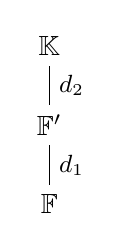
\begin{tikzpicture}
            %Nodes
            \node at (0,-1) (F) {$\F$};
            \node at (0,0) (F') {$\F'$};
            \node at (0,1) (K) {$\K$};

            %Lines
            \draw (F) -- (F') node[midway, right] {\small $d_1$};
            \draw (F') -- (K) node[midway, right] {\small $d_2$};
        \end{tikzpicture}
    \end{center}
    Let $m_{\alpha_{n+1}} \in \F'[x]$ be the minimal polynomial of $\alpha_{n+1}$, then $\deg m_{\alpha_{n+1}} = [\K : \F'] = d_2$. We can easily notice that any element of $\Hom_{\F}(\K, \E)$ restricted to $\F'$ is an element of $\Hom_{\F}(\F', \E)$. Hence, to have an estimation on the size of $\Hom_{\F}(\K, \E)$, we can determine in how many ways each element of $\Hom_{\F}(\F', \E)$ can be extended to an element of $\Hom_{\F}(\K, \E)$. By Theorem \ref{master theorm roots minimal and homomorphisms}, we have that each $\varphi_0$ in $\Hom_{\F}(\F', \E)$ can be extended in at most $\deg m_{\alpha_{n+1}}^{\varphi_0} = \deg m_{\alpha_{n+1}} = d_2$ ways. Therefore, since there are at most $d_1$ elements in $\Hom_{\F}(\F', \E)$, then by the multiplicativity of the degree:
    $$\#\Hom_{\F}(\K, \E) \leq d_1 d_2 = [\F': \F] [\K : \F'] = [\K : \F].$$
    This concludes our proof by induction. To prove the actual claim, notice that since $\E$ is a finite extension, then it can be written as $\F(\alpha_1, ..., \alpha_n)$ where $\alpha_1, ..., \alpha_{[\E : \F]}$ is the basis of $\E$ as a $\F$-vector space. Therefore, we can plug-in $\K = \E$ to get
    $$\# \Aut(\E / \F) = \# \Hom_{\F}(\E, \E) \leq [\E : \F]$$
    which proves our claim. 
\end{proof}

\subsection{Galois Extensions} \label{galois_extensions}

Theorem \ref{upperbound for automorphism group}, shows that there are at most $[\E : \F]$ automorphisms in the automorphism group of a finite extension. Is it possible to prove that there in fact exactly  $[\E : \F]$ automorphisms in the automorphism group ? To answer this question, consider the situation where $\E$ is generated by a single element $\alpha$, then $[\E : \F]$ is equal to the degree of the minimal polynomial of $\alpha$. By Theorem \ref{roots minimal polynomial and automorphisms}, we know that there are as much automorphisms as roots of the minimal polynomial in $\E$. Thus, if the minimal polynomial of $\alpha$ doesn't factor completely into linear terms in $\E$, then $\#\Aut(\E / \F) < [\E : \F]$.

This happens for example when $\F = \Q$ and $\E = \Q(\sqrt[3]{2})$. The minimal polynomial of $\sqrt[3]{2}$ in $\Q(\sqrt[3]{2})$ is $x^3 - 2 \in \Q[x]$. The two other roots of the minimal polynomial are complex numbers so $\sqrt[3]{2}$ is the only roots of its minimal polynomial in $\Q(\sqrt[3]{2})$. Therefore, $\#\Aut(\Q(\sqrt[3]{2}) / \Q) < [\Q(\sqrt[3]{2}) : \Q]$. This shows that $\Aut(\E / \F) = [\E : \F]$ may not always hold. However, we are very interested in the situations where this equation holds since it can be used to deduce a lot of informations about the extension.

\begin{definition}[Galois Extensions]
    A finite field extension $\E / \F$ is a Galois extension if $\# \Aut(\E / \F) = [\E : \F]$. In that case, we write $\Gal(\E / \F)$ to mean $\Aut(\E / \F)$.
\end{definition}

When $\E = \C$ and $\R$, then $[\E : \F] = 2$. Moreover, beside the identify automorphism, the conjugation map is also an automorphism of $\C / \R$. By Theorem \ref{upperbound for automorphism group}, these must be the only automorphisms of $\C / \R$. It follows that $[\C : \R] = 2$ and so $\C / \R$ is a Galois extension.

As before, consider the extension $\Q(\sqrt[3]{2})$ of $\Q$ of degree 3. We already showed that it is not a Galois extension since the extension only contains one root of the minimal polynomial of $\sqrt[3]{2}$. Let $\zeta$ be a cube root of 1 distinct than 1, then the minimal polynomial of $\zeta$ over $\Q$ can be found by writing
$$\zeta^3 - 1 = 0 \implies (\zeta - 1)(\zeta^2 + \zeta + 1) = 0 \implies \zeta^2 + \zeta + 1 = 0$$
and noticing that $x^2 + x + 1$ is irreducible over $\Q$ (since it is irreducible over $\R$). It follows that the minimal polynomial of $\zeta$ is $p(x) = x^2 + x + 1$. Hence, $\Q(\zeta) \subset \C$ is an extension of $\Q$ of degree $2$. Similarly, if we consider the extension $\Q(\sqrt[3]{2}, \zeta) = \Q(\sqrt[3]{2})(\zeta)$ of $\Q(\sqrt[3]{2})$, then $p$ stays irreducible so this extension also has degree 2. Therefore, by the following diagram and by the multiplicativity of the degree, $\Q(\sqrt[3]{2}, \zeta)$ is an extension of $\Q(\zeta)$ of degree 2:
\begin{center}
    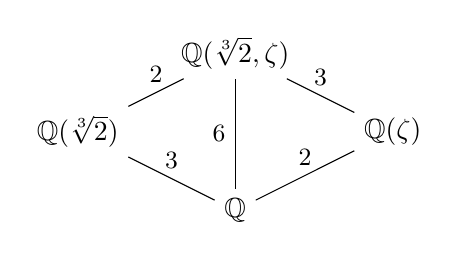
\begin{tikzpicture}
        %Nodes
        \node at (0,-1) (Q) {$\Q$};
        \node at (-2,0) (Qs) {$\Q(\sqrt[3]{2})$};
        \node at (2,0) (Qz) {$\Q(\zeta)$};
        \node at (0,1) (Qsz) {$\Q(\sqrt[3]{2}, \zeta)$};

        %Lines
        \draw (Q) -- (Qs) node[midway, above] {\small $3$};
        \draw (Q) -- (Qz) node[midway, above] {\small $2$};
        \draw (Q) -- (Qsz) node[midway, left] {\small $6$};
        \draw (Qs) -- (Qsz) node[midway, above] {\small $2$};
        \draw (Qz) -- (Qsz) node[midway, above] {\small $3$};
    \end{tikzpicture}
\end{center}
Let's count the number of elements in $\Aut(\Q(\sqrt[3]{2}, \zeta) / \Q)$. Let $\phi \in \Aut(\Q(\sqrt[3]{2}, \zeta) / \Q)$, then $\varphi(\zeta)$ must be a root of $x^2 + x + 1$ so $\varphi(\zeta)$ can be mapped to $\zeta$ and $\overline{\zeta}$. Similarly, $\sqrt[3]{2}$ must be mapped to a root of $x^3 - 2$. But since $\zeta^3 = 1$, then $\varphi(\sqrt[3]{2})$ can be $\sqrt[3]{2}$, $\zeta\sqrt[3]{2}$ or $\overline{\zeta} \sqrt[3]{2}$. Since $\varphi$ is only determined by $\varphi(\zeta)$ and $\varphi(\sqrt[3]{2})$, then there are 6 elements in $\Aut(\Q(\sqrt[3]{2}, \zeta) / \Q)$. Therefore, it is a Galois extension. 


Let's determine the structure of $G = \Gal(\Q(\sqrt[3]{2}, \zeta) / \Q)$. Since it has cardinality 6, then it is either $\Zn{6}$ or $S_3$. Let's show that it is $S_3$ by showing that no element has order 6. Let $\varphi \in G$, if $\varphi(\zeta) = \zeta$ or $\varphi(\sqrt[3]{2}) = \sqrt[3]{2}$, then $\varphi$ has at most order 3. Hence, the only possible candidates for an element of order 6 in $G$ are $\varphi_1$ and $\varphi_2$ where $\varphi_1(\zeta) = \varphi_2(\zeta) = \overline{\zeta}$, $\varphi_1(\sqrt[3]{2}) = \zeta \sqrt[3]{2}$ and $\varphi_2(\sqrt[3]{2}) = \overline{\zeta} \sqrt[3]{2}$. Notice that in both cases, $\overline{\zeta}$ is mapped to $\zeta$ because it can only be mapped to a root of $x^2 + x + 1 = (x - \zeta)(x - \overline{\zeta})$ and if it was mapped to $\overline{\zeta}$, then it would break the fact that it is injective. Hence,
$$\varphi_1^2(\zeta) = \varphi_1(\overline{\zeta}) = \zeta \quad \text{ and }\quad \varphi_1^2(\sqrt[3]{2}) = \varphi_1(\zeta)\varphi_1(\sqrt[3]{2}) = \overline{\zeta}\zeta \sqrt[3]{2} = \sqrt[3]{2}$$
and 
$$\varphi_2^2(\zeta) = \varphi_2(\overline{\zeta}) = \zeta \quad \text{ and }\quad \varphi_2^2(\sqrt[3]{2}) = \varphi_2(\overline{\zeta})\varphi_2(\sqrt[3]{2}) = \zeta \overline{\zeta} \sqrt[3]{2} = \sqrt[3]{2}$$
so $\varphi_1^2 = \varphi_2^2 = id$. Thus, both $\varphi_1$ and $\varphi_2$ have order 2. It follows that $G$ has no element of order 6 so $G$ must be $S_3$.


Galois Extensions can be seen as field extensions on which we can read off a lot of structure and properties from the symmetries. The next theorem justifies this way of thinking about Galois extensions. In the next propositions and definitions, fix a field $\F$, a finite Galois extension $\E$ and denote by $G$ the Galois Group of $\E / \F$. \\

\begin{notation}
    $\E^G = \{\alpha \in \E : g(\alpha) = \alpha \text{ for all } g\in G\}$ is the set of fixed points of $G$.
\end{notation}

\begin{lemma}
\label{lemma : fixed points is a subfield of E containing F}
    $\E^G$ is a subfield of $\E$ which contains $\F$.
\end{lemma}

\begin{proof}
    All the elements of $\F$ are fixed by all the elements of $G$ so $\F \subset \E^G$. Moreover, by definition, we already know that $\E^G \subset \E$. Hence, it remains to show that $\E^G$ is a subfield of $\E$, i.e., that $\E^G$ contains 0, 1, is closed under addition, multiplication and respective inverses. Since $\F \subset \E^G$, then in particular $0,1 \in \E^G$. Since the elements of $G$ are field homomorphisms, then for all $x,y \in \E^G$ and $\varphi \in G$, we have $\varphi(x + y) = \varphi(x) + \varphi(y) = x + y$ and $\varphi(xy) = \varphi(x)\varphi(y) = xy$ so $\E^C$ is closed under addition and multiplication. Similarly, for all $x,y \in \E^G$ with $y \neq 0$ and $\varphi \in G$, we have $\varphi(-x) = -\varphi(x) = -x$ and $\varphi(y^{-1}) = \varphi(y)^{-1} = y^{-1}$ so $\E^G$ is closed under additive and multiplicative inverses. Therefore, $\E^G$ is a subfield of $\E$.
\end{proof}

\begin{theorem}
\label{fixed points is ground field of galois}
    $\E^G = \F$.
\end{theorem}

\begin{proof}
    By the previous lemma, we have the following tower of extensions
    \begin{center}
        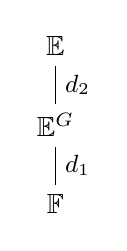
\begin{tikzpicture}
            %Nodes
            \node at (0,-1) (F) {$\F$};
            \node at (0,0) (F') {$\E^G$};
            \node at (0,1) (K) {$\E$};

            %Lines
            \draw (F) -- (F') node[midway, right] {\small $d_1$};
            \draw (F') -- (K) node[midway, right] {\small $d_2$};
        \end{tikzpicture}
    \end{center}
    where $d_1 = [\E^G : \F]$ and $d_2 = [\E : \E^G]$. Let's show that $d_1 = 1$. Consider the set $\Aut(\E / \E^G)$, then it must contain $G$. Moreover, by the last theorem of the previous section, $\# \Aut(\E / \E^G) \leq d_2 = [\E : \E^G] \leq [\E : \F]$. Thus, we obtain:
    $$[\E : \F] = \# G \leq \# \Aut(\E / \E^G) \leq [\E : \F]$$
    which implies that $\# \Aut(\E / \E^G) = [\E : \E^G] = d_1 d_2 \leq d_2$. It follows that $d_1 = 1$. 
\end{proof}

By Theorem \ref{roots minimal polynomial and automorphisms}, the minimal polynomial of $\alpha$ in a Galois extension of the form $\F(\alpha)$ must split completely into linear factors. It turns out that this can be generalized to any irreducible polynomial with a root in the Galois extension.

\begin{theorem}
\label{galois implies normal}
    If $f$ is an irreducible polynomial in $\F[x]$ which has a root in $\E$, then $f$ splits completely into linear factors in $\E[x]$. 
\end{theorem}

\begin{proof}
    Let $r \in \E$ be a root of $f$, then it is easy to see that $f$ is the minimal polynomial of $r$ over $\F$. Consider the orbit $\{r_1, ..., r_n\}$ of $r$ under the action of $G$ on $\E$ and define the polynomial $g(x) = \prod(x - r_i) \in \E[x]$. Notice that if we expand the product, we get that $g(x) = x^n - \sigma_1 x^{n - 1} + ... + (-1)^n \sigma_n$ where the $\sigma_i$'s are the elementary symmetric functions in $r_1, ..., r_n$. It follows that for all $1 \leq i \leq n$, $\sigma_i \in \E^G = \F$ since by symmetry $\sigma_i$ is fixed by all the elements of $G$. Thus, $g \in \F[x]$ with $g(r) = 0$ so it follows by minimality of $f$ that $f$ divides $g$. Therefore, in $\E[x]$, $f$ divides a product of linear factors so $f$ must itself be a product of linear factors. Hence, $f$ splits completely in $\E[x]$. 
\end{proof}

If a field extension has the property that any irreducible polynomial in the polynomial ring of the ground field with a root in the extension splits completely in the polynomial ring of the extension, we say that the extension is normal. Using this terminology, the previous theorem states that any Galois extension is normal.

\section{Splitting Fields} \label{splitting_fields}

\subsection{Existence and Uniqueness}

As we saw in the last section, an interesting property of Galois extensions is the way polynomials in the ground field splits in the Galois extension. In this section, we will explore in more details these situations with the notion of a splitting field, and we will then see how it relates to Galois extensions.

\begin{definition}
    Given a field $\F$ and a polynomial $f \in \F[x]$, a splitting field of $f$ is an extension $\E / \F$ satisfying
    \begin{enumerate}[label=(\alph*)]
        \item $f$ factors into linear factors in $\E[x]$.
        \item $E$ is generated as a field by the roots $r_1, ..., r_n$ of $f$.
    \end{enumerate}
\end{definition}

With this definition, it is not clear, even if it might be easy to guess, that such fields always exist. The following theorem answers this matter.

\begin{theorem}[Existence]
    Given a field $\F$ and a polynomial $f$, there exists an extension $\E / \F$ which is a splitting field of $f$.
\end{theorem}

\begin{proof}
    Let's prove it by induction on the degree of $f$. For the base case, $n=1$, if $f$ has degree 1, then its unique root $r$ must be in $\F$ already so $\E = \F(r) = \F$ is a splitting field of $f$. For the Inductive Step, assume that the statement holds for polynomials of degree $n$ and suppose that $f$ has degree $n+1$. Let $p$ be an irreducible factor of $f$ and construct the field $L = \F[x]/(p) = \F(r_0)$ which contains a root $r_0$ of $p$. It follows that $f(x)$ can be written as $(x - r)g(x)$ in $L[x]$ where $g$ has degree $n$. Hence, by applying the inductive hypothesis, we can construct a splitting field $\E / L$ of $g$. It follows that $g(x)$ can be written as $(x - r_1) \dots (x - r_n)$ in $\E[x]$ so $f(x)$ splits completely into $(x - r_0)(x - r_1) \dots (x - r_n)$ in $\E[x]$. Moreover, since $\E$ is generated by $L$ and the roots of $g$, then
    $$\E = L(r_1, ..., r_n) = \F(r_0)(r_1, ..., r_n) = \F(r_0, r_1, ..., r_n)$$
    which proves that $\E$ is generated by the roots of $f$. Therefore, by induction, we can always construct a splitting field given a field $\F$ and a polynomial $f \in \F[x]$.
\end{proof}

It is very hard to compute the degree of a splitting field since it depends very subtly on the structure of $f$. However, by the multiplicativity of the degree, the degree of the splitting field must be smaller than $(\deg f)!$. For now, we proved that a splitting field must exist for a field $\F$ and polynomial $f \in \F[x]$, but it turns out that splitting fields of $f$ are isomorphic as field extensions. Let's state it properly and prove it.

\begin{theorem}[Uniqueness]
    Given a field $\F$, a polynomial $f \in \F[x]$ and two splitting fields $\E$ and $\E'$ of $f$ over $\F$, then $\E$ and $\E'$ are isomorphic as extensions of $\F$, i.e., there exists a field isomorphism from $\E$ to $\E'$ that fixes $\F$.
\end{theorem}

\begin{proof}
    Let's proceed by induction on $n = \deg f$. For the base case, if $\deg f = 1$, then we simply have $\E = \F = \E'$ so we are done. Assume now that the claim holds for $n$ and suppose that $\deg f = n+1$. Let $p \in \F[x]$ be an irreducible factor of the polynomial $f$, let $r$ be a root of $p$ in $\E$ and let $r'$ be a root of $p$ in $\E'$. We have the following diagram:
    \begin{center}
        \begin{tikzpicture}
            %Nodes
            \node at (0,-1.5) (F) {$\F$};
            \node at (-1.5,0) (Fr) {$\F(r)$};
            \node at (-1.5,1.5) (E) {$\E$};
            \node at (1.5,0) (Fr') {$\F(r')$};
            \node at (1.5,1.5) (E') {$\E'$};

            %Lines
            \draw (F) -- (Fr);
            \draw (F) -- (Fr');
            \draw (Fr) -- (E);
            \draw (Fr') -- (E');
            \draw [dashed, ->] (Fr) -- (Fr') node[midway, above] {\small $\varphi$};
        \end{tikzpicture}
    \end{center}
    Notice that both $\F(r)$ and $\F(r')$ are isomorphic to $\F[x]/(p)$ so in particular, $\F(r) \isomorphic \F(r')$. Let $\varphi : \F(r) \to \F(r')$ be such an isomorphism. Hence, if we let $L = \F(r) = \F(r')$, our diagram becomes
    \begin{center}
        \begin{tikzpicture}
            %Nodes
            \node at (0,-1.5) (F) {$\F$};
            \node at (0,0) (L) {$L$};
            \node at (-1.5,1.5) (E) {$\E$};
            \node at (1.5,1.5) (E') {$\E'$};

            %Lines
            \draw (F) -- (L);
            \draw (L) -- (E);
            \draw (L) -- (E');
        \end{tikzpicture}
    \end{center}
    It follows that $\E$ and $\E'$ can be seen of splitting fields of a polynomial in $L[x]$ of degree $n$ so by the inductive hypothesis, $\E$ and $\E'$ are isomorphic as extensions of $L$. Therefore, $\E$ and $\E'$ are isomorphic as extensions of $\F$. 
\end{proof}

We can now talk about \textit{the} splitting field of a polynomial $f$ over a field $\F$. The next theorem justifies the link between splitting fields and Galois extensions. 

\begin{proposition}
\label{Galois implies splitting field}
    If $\E / \F$ is a Galois extension, then $\E$ is the splitting field of a polynomial $f \in \F[x]$.
\end{proposition}

\begin{proof}
    Since $[\E : \F] < \infty$, then we can let $\alpha_1, ..., \alpha_n$ be a finite set of generators for $\E / \F$. Since every element of $\E$ is algebraic over $\F$, then we can let $f_1, ..., f_n$ be irreducible polynomials in $\F[x]$ having respective roots $\alpha_1, ..., \alpha_n$ and define $f = f_1 \cdot \dots \cdot f_n$. In $\E[x]$, all the $f_i$'s factor completely by Theorem \ref{galois implies normal} and therefore so does $f$. Moreover, the roots of $f$ in $\E$ generate $\E$ so $\E$ is the splitting field of $f$ over $\F$.
\end{proof}

\subsection{Application to Finite Fields} \label{application to finite fields}

Recall that if $\F$ is a finite field, then it must have characteristic equal to a prime number $p$ (Theorem \ref{characteristic prime}) which implies that $\F$ contains a copy of $\F_p$. From this, we can see $\F$ as a vector space over $\Zn{p}$ which implies that $\#\F$ must be a power of $p$. However, given any prime power $p^n$ can we construct fields of cardinality $p^n$ ? Are they necessarily isomorphic one to another ?

\begin{theorem}
    Given a prime $p$ and a natural number $n$, there is a unique field of cardinality $p^n$ up to isomorphism.
\end{theorem}

One possible approach would be to find a polynomial $f \in \F_p[x]$ which is irreducible of degree $n$ and construct $\F = \F_p[x] / (f)$ which is the desired field. However, it is not clear that there exists such a polynomial $f$ or there might be several of them. We will not use this approach in the proof. The theory of splitting fields we developed gives us the perfect tools to prove this theorem. 

\begin{proof}
    Let $\F$ be the splitting field of $f(x) = x^{p^n} - x \in \F_p[x]$, let's show that $\F$ has cardinality $p^n$. First, notice that $f$ has distinct roots in $\F$ since its formal derivative is identically $-1$ (so no multiple roots by Theorem \ref{formal derivatives and multiple roots}). Since $f$ splits completely in $\F$, then $f$ has $p^n$ roots $\alpha_1, ..., \alpha_{p^n}$. But notice that the roots of $f$ in $\F$ form a field which contains $\F_p$. It follows that $\F = \F_p(\alpha_1, ..., \alpha_{p^n})$ is simply the set of roots of $f$ in $\F$. Therefore, $\F$ has cardinality $p^n$ which proves the existence part of the claim.
    
    Now, let $\F'$ be a field of cardinality $p^n$, then $\F'$ must have characteristic $p$ (because we know that $\# \F' = q^m$ where $q$ is its characteristic which is a prime number, $q^m = p^n \implies \text{char}(\F') = p$). It follows that $\F'$ contains $\F_p$ as a subfield so it is an extension of $\F_p$. Moreover, notice that all the elements of $\F'$ are roots of the polynomial $f(x) = x^{p^n} - x \in \F_p[x]$ so $f$ splits completely in $\F'$ (since $\# \F' = \deg f$). And finally, since the elements of $\F'$ are precisely the roots of the $f$, then we can say that $\F'$ is generated by the roots of $f$. It follows that $\F'$ is the splitting field of $f$ over $\F$. By uniqueness of the splitting field, we have that $\F' \isomorphic \F$. Since every field of cardinality $p^n$ is isomorphic to $\F$, then the field of cardinality $p^n$ is unique up to isomorphism. 
\end{proof}

Let's now determine if $\F_q$ (where $q = p^n$) is a Galois extension of $\F_p$. To do so, we need to determine the number of automorphisms in the automorphism group $\Aut(\F_q / \F_p)$. To understand this group, we will heavily rely on the important observation that in $\F_q$, $(x + y)^p = x^p + y^p$. This equation means that taking the $p$th power is not only well-behaved for multiplication but also for addition in $\F_q$. This motivates the following proposition and definition.

\begin{proposition}
    The map $\F_q \to \F_q : x \mapsto x^p$ is an automorphism.
\end{proposition}

\begin{proof}
    First, notice that this map trivialy preserves multiplication but also preserves addition by our previous discussion. Hence, it remains to show that it fixes $\F_p$. To see why it is the case, recall Fermat's Little Theorem which states that for any $x \in \F_p^{\times}$, $x^{p-1} = 1$. Multiplying by $x$ on both sides gives us $x^p = x$ for all $x \in \F_p^{\times}$. Since this equation also holds for $x = 0$, then the map fixes $F_p$. 
\end{proof}

\begin{definition}
    The map $\varphi : \F_q \to \F_q$ defined by $x \mapsto x^p$ is called the Frobenius Automorphism. Indeed, by the previous proposition, $\varphi \in \Aut(\F_q / \F_p)$.
\end{definition}

The Frobenius Automorphism, gives us a concrete element in $\Aut(\F_q / \F_p)$. This lets us understand the group $\Aut(\F_q / \F_p)$ as shown by the following theorem where the Frobenius Automorphism plays a crucial role. 

\begin{theorem}
    $F_q$ is a Galois extension of $\F_p$. The Galois Group of the extension is $\Zn{n}$ and is generated by the Frobenius Automorphism.
\end{theorem}

\begin{proof}
    First, we already have that $\Aut(\F_q / \F_p)$ is finite since $\#\Aut(\F_q / \F_p) \leq [\F_q : \F_p] = n$. Let's find the order of the Frobenius Automorphism $\varphi$, which must be finite by the previous observation. For all $k \in \N$, we have that $\varphi^k(x) = x^{p^k}$. Moreover, since $\F_q^{\times}$ is cyclic and of order $p^n - 1$, then there is a $\alpha \in \F_q$ such that $\alpha^{p^n} = \alpha$ but $\alpha^{p^k} \neq \alpha$ for all $k < n$. Hence, if we denote by $k_0$ the order of $\varphi$, then we must have $\varphi^{k_0} = id$ and in particular $\alpha^{p^{k_0}} = \varphi^{k_0}(\alpha) = \alpha$. It follows that $k_0$ must be at least greater than or equal to $n$. Moreover, since $\F_q^{\times}$ has $p^{n} - 1$ elements, then $x^{p^n - 1} = 1$ for all $x \in \F_q^{\times}$. Equivalently, $\varphi^n(x) = x^{p^n} = x$ for all $x \in \F_q$. Thus, $k_0$ must be smaller than $n$. Therefore, $k_0$ so $\varphi$ has order $n$. We obtain the following inequality:
    $$n = \# \langle \varphi \rangle \leq \# \Aut(\F_q / \F_p) \leq n$$
    which lets us conclude that $\# \Aut(\F_q / \F_p) = [\F_q : \F_p]$. Therefore, $\F_q / \F_p$ is a Galois extension and its Galois group is cyclic, generated by the Frobenius Automorphism, and hence, isomorphic to $\Zn{n}$.
\end{proof}

\subsection{Characterizing Galois Extensions} \label{characterizations of galois extensions}

For the moment, our definition of Galois extensions only applies to finite extensions. However, there is a way of extending this definition to infinite extensions by finding an equivalent definition of Galois extensions that doesn't rely on the finiteness of the degree. Recall that at the end of Section \ref{galois_extensions}, we proved that any Galois extension is normal. Let's improve it this result and use it to characterize Galois extensions.

\begin{definition}[Normal Extension]
    An extension $\E / \F$ is normal if every irreducible polynomial in $\F[x]$ with a root in $\E$ splits into linear factors in $\E[x]$.
\end{definition}

As we will see, the converse of Theorem \ref{galois implies normal} is not true. However, we can make it true by adding another assumption on the extension.

\begin{definition}[Separability]
    An extension $\E / \F$ is separable if every irreducible polynomial with a root in $\E$ has no multiple roots.
\end{definition}

The next theorem shows that the seperability of an extension comes for free most of the time since the main applications and examples of this theory is to fields of characteristic zero.

\begin{proposition}
    If $\F$ has characteristic 0, then every extension of $\F$ is separable.
\end{proposition}

\begin{proof}
    Let $f \in \F[x]$ be an irreducible polynomial with a root $r \in \E$ and suppose that $f(x) = (x - r)^eg(x)$ in $\E[x]$ with $\gcd((x - r), g(x)) = 1$. Consider the formal derivative $f'$ of $f$ and notice that if $e > 1$, then $r$ is again a root of $f'$ by Theorem \ref{formal derivatives and multiple roots}. Hence, $r$ is a root of $\gcd(f, f') \in \F[x]$.
    $$f(x) = a_n x^n + ... + a_1x + a_0 \quad \text{ and } \quad f'(x) = na_n x^{n-1} + ... + a_1$$
    Recall that $f$ is irreducible in $\F[x]$ so $\gcd(f,f')$ is either $f$ or 1 since it divides $f$. But since $\gcd(f,f')$ also divides $f'$ which has degree $n-1$, then $\gcd(f,f') = 1$. Therefore, by contradiction, $e = 1$ so $\alpha$ is not a multiple root.
\end{proof}

The assumption that $\F$ has characteristic 0 was used when asserting that $\deg f' = n-1$. If $\F = \F_p$ for a prime $p$ and $f(x) = x^p$, then $\deg f' = 0$ so $\gcd(f, f') = f$. When the field doesn't have characteristic zero, then computing the degree of the formal derivative is not as easy.

\begin{theorem}
\label{Galois implies normal and separable}
    If $\E / \F$ is Galois, then it is normal and separable.
\end{theorem}

\begin{proof}
    Let $f \in \F[x]$ be an irreducible polynomial and $r \in \E$ be a root of $f$. Consider the orbit $r_1, ..., r_n$ of $r$ under the action of the Galois group and define the polynomial $g(x) = (x-r_1)...(x-r_n) \in \E[x]$. If we expand the product which defines $g$, we get that the coefficients in front of the powers of $x$ are the elementary symmetric polynomials in $r_1, ..., r_n$. Since the $r_i$'s are in the same orbit under the action of the Galois group, then the coefficients are all fixed by every element of the Galois group, thus, they are in $\F$. It follows that $g$ is a polynomial on $\F$ for which $r$ is a root. 
    
    Since $r$ is a root of the irreducible polynomial $f$, then $f$ must be the minimal polynomial of $r$. Since $g$ is a polynomial in $\F[x]$ for which $r$ is a root, then $f$ must divide $g$. It follows that on $\E$, $f$ must split into distinct linear factors since $g$ can be completely split into distinct linear factors. Since it holds for all $f \in \F[x]$ irreducible with a root in $\E$, then $\E / \F$ must be both normal and separable.
\end{proof}

It turns out that the converse is also true and the proof is very similar to the proof of Theorem \ref{upperbound for automorphism group} with some additional assumptions that replace inequalities with equalities.

\begin{theorem}
\label{normal separable implies Galois}
    If $\E / \F$ is finite, normal and separable, then $\E / \F$ is Galois.
\end{theorem}

\begin{proof}
    Let's prove by strong induction on the degree that $\# \Hom_{\F}(\K, \E) = [\K : \F]$ where $\K \subset \E$ is a finite field extension of $\F$. Notice that the base case $[\K : \F] = 1$ is trivial since in that case, $\K = \F$ and so the only automorphism is the identity. 
    
    Suppose now that there is a $n$ such that any extension of $\F \subset \K \subset \E$ of degree strictly smaller than $n$ satisfies $\# \Hom_{\F}(\K, \E) = [\K : \F]$. Let $\K \subset \E$ be an extension of $\F$ of degree $n$ and notice that either $\K$ is of the form $\F(\alpha)$ or of the form $\F'(\alpha)$ for some extension $\F'$ of $\F$ different from $\F$. Let's show that in both cases, the equation $\# \Hom_{\F}(\K, \E) = [\K : \F]$ holds.
    
    If $\K = \F(\alpha)$, then the degree of $\K / \F$ is simply the degree of the minimal polynomial $m_{\alpha}$ of $\alpha$. By Theorem \ref{master theorm roots minimal and homomorphisms}, we have that 
    $$\# \Hom_{\F}(\K, \E) = \#\{\text{roots of } m_{\alpha} \text{ in } \E\}.$$
    But since $\E$ is normal and separable, then $m_{\alpha}$ splits completely into distinct linear factors and so the number of roots of $m_{\alpha}$ in $\E$ is simply equal to $\deg m_{\alpha}$. Therefore, $\# \Hom_{\F}(\K, \E) = [\K : \F]$.

    If $\K = \F'(\alpha)$ with $\alpha \notin \F'$ and $\F' \neq \F$, then the degree of $\F'/\F$ must be strictly smaller than $n$ and so by the induction hypothesis, $\# \Hom_{\F'}(\F', \E) = [\K : \F]$. By Theorem \ref{master theorm roots minimal and homomorphisms}, the elements in $\Hom_{\F}(\K, \E)$ are all extensions of elements in $\Hom_{\F}(\F', \E)$. Let $\varphi_0 \in \Hom_{\F}(\K, \E)$, then by the same theorem, $\varphi_0$ has as much extensions in $\Hom_{\F}(\K, \E)$ as there are roots of $m_{\alpha}^{\varphi_0}$ in $\E$. Let's show that $m_{\alpha}^{\varphi_0}$ splits into distinct linear factors in $\E[x]$. If we let $m \in \F[x]$ be the minimal polynomial of $\alpha$ over $\F$, we get that $m_{\alpha}$ divides $m$. It follows that $m_{\alpha}^{\varphi_0}$ divides $m^{\varphi_0}$. But since $m$ has coefficients in $\F$ and $\varphi_0$ fixes the elements of $\F$, then $m^{\varphi_0} = m$. Hence, $m_{\alpha}^{\varphi_0}$ divides $m$. Since $\E$ is normal and separable, then $m$ must split completely into distinct linear factors and so does $m_{\alpha}^{\varphi_0}$. Thus, $m_{\alpha}^{\varphi_0}$ has as much roots in $\E$ as its degree. But notice that $\deg m_{\alpha}^{\varphi_0} = \deg m_{\alpha} = d_2$ so $\varphi_0$ has exactly $d_2$ extensions. It follows that 
    $$\#\Hom_{\F}(\K, \E) = \#\Hom_{\F}(\F', \E) \times d_2 = d_1 d_2 = [\K : \F].$$
    By induction, it holds for all finite extensions $\K$. In particular, it holds for $\K = \E$ which gives us 
    $$\#\Aut(\E / \F) = [\E : \F].$$ 
    Therefore, $\E$ is a Galois extension.
\end{proof}

We have found a characterization of Galois extensions as desired at the beginning of the subsection. With this characterization, we can actually deduce a second one. The next theorem summarizes these characterizations into one place.

\begin{theorem}
\label{theorem characterizations of Galois}
    If $\E / \F$ is a finite extension, then TFAE:
    \begin{enumerate}
        \item $\E / \F$ is a Galois extension.
        \item $\# \Aut(\E / \F) = [\E : \F]$
        \item $\E$ is normal and separable over $\F$.
        \item $\E$ is the splitting field of a separable polynomial over $\F$.
    \end{enumerate}
\end{theorem}

\begin{proof}
    Property 1 and 2 are equivalent by definition and Property 1 and 3 are equivalent by Theorem \ref{Galois implies normal and separable} and Theorem \ref{normal separable implies Galois}. By Proposition \ref{Galois implies splitting field}, Property 1 implies that $\E$ is the splitting field of a polynomial, however, we didn't prove that this polynomial is separable. Let's prove it by going over the proof of the proposition. Since $[\E : \F] < \infty$, then we can let $\alpha_1, ..., \alpha_n$ be a finite set of generators for $\E / \F$. Let the $f_i$'s be the respective minimal polynomials of the $\alpha_i$'s and define $f = f_1 \cdot \dots \cdot f_n$ such that the $f_i$'s are distinct: if $f_i$ and $f_j$ are equal, simply remove one of them. In $\E[x]$, all the $f_i$'s factor completely by normality and therefore so does $f$. Moreover, the roots of $f$ in $\E$ generate $\E$ so $\E$ is the splitting field of $f$ over $\F$. To show that $f$ is separable, suppose that it has a multiple root. By separability of $\E$, the $f_i$'s cannot have multiple roots so it must be that $\gcd(f_i, f_j) \neq 1$ for some $i$ and $j$. Since both are irreducible, then $f_i = \gcd(f_i, f_j) = f_j$ which is in contradiction with our construction of $f$. Therefore, $\E$ is the splitting field of a separable polynomial.
    
    Let's now prove that Property 4 implies one of Property 1, 2 or 3 to finish the proof. Suppose that $\E$ is the splitting field of a separable polynomial, then $f$ splits completely into distinct linear factors. Moreover, $\E$ is generated by the roots of $f$. Notice that in the proof of Theorem \ref{normal separable implies Galois}, the assumption that the extension is normal and separable was here to make sure that the generators are roots of polynomials that splits completely into distinct linear factors. We don't need this assumption anymore since it now follows from the fact that $\E$ is the splitting field of a separable polynomial. Therefore, if rework the proof of Theorem \ref{normal separable implies Galois}, we obtain that $\E$ is Galois. Therefore, Property 4 implies Property 1.
\end{proof}

Since Property 2 in the previous theorem also makes sense for infinite extensions, we can now define what it means for an infinite extension to be Galois even though it will not be useful for us here.

\begin{definition}
    An extension  $\E / \F$ (not necessarily finite) is said to be Galois if it is normal and separable over $\F$.
\end{definition}

All the applications of Galois Theory that we will explore at the end of these notes will concern finite extensions but it is still good to keep in mind this new definition.

\section{The Galois Correspondence} \label{galois_correspondence}

\subsection{The Fundamental Theorem of Galois Theory}

The Galois Correspondence is really the Fundamental Theorem of Galois Theory. This theorem makes a connection between the subgroups of the Galois group and the subfields of the Galois extension. It turns out that there is a very deep connection that will let us understand the structure of Galois extensions. However, to prove it, we will need to prove a bunch of theorems first.

\begin{proposition}
\label{galois extension is galois over subfields}
    If $\E / \F$ is a finite Galois extension and $\K$ is a subfield of $\E$ containing $\F$, then $\E$ is Galois over $\K$.
\end{proposition}

\begin{proof}
    By Theorem \ref{theorem characterizations of Galois}, we have that $\E$ is normal and separable over $\F$. Let's show that $\E$ is normal and separable over $\K$. Let $p \in \K[x]$ be an irreducible polynomial which has a root $\alpha$ in $\E$, then $p$ is the minimal polynomial of $\alpha$ over $\K$. If we let $m_{\alpha} \in \F[x]$ be the minimal polynomial of $\alpha$ over $\F$, then $p$ divides $m_{\alpha}$. By normality and separability of $\E$ over $\F$, $m_{\alpha}$ splits completely into distinct linear factors over $\E$ and so does $p$. Therefore, $\E$ is normal and separable over $\K$, so it follows from Theorem \ref{theorem characterizations of Galois} that $\E$ is Galois over $\K$.
\end{proof}

Here is a second proof which uses the theory of Group Actions.

\begin{proof}
    Let $G = \Gal(\E / \F)$ and $X = \Hom_{\F}(\K, \E)$, then we know by the proof of Theorem \ref{normal separable implies Galois} that $\#X = [\K : \F]$. But notice that $X$ can be seen as a $G$-set where $G$ acts by composition. This action is transitive since for all $\varphi_1, \varphi_2 \in X$, we have that $\varphi_1 \circ \varphi_2^{-1}$ can be extended to an element in $G$ and so there is a $\sigma$ such that $\sigma \varphi_2 = \varphi_1$. Thus, by the Orbit-Stabilizer Theorem, $\#X \# \text{Stab}(id) = \# G$ which is equivalent to $[\K : \F] \# \text{Stab}(id) = [\E : \F]$. By the multiplicativity of the degree, we obtain that $\# \text{Stab}(id) = [\E : \K]$. Now, notice that the stabilizer of the identity is precisely $\Aut(\E / \K)$. Thus, $\# \Aut(\E / \K) = [\E : \K]$ which proves that $\E$ is Galois over $\K$. 
\end{proof}

In subsection \ref{application to finite fields}, we showed that any finite extension $\E$ of $\F_p$ is Galois with a cyclic Galois group generated by the Frobenius automorphism $\delta : x \mapsto x^p$. If $\F \subset \K \subset \E$, then $\K = \F_{p^t}$ and so by the previous theorem, $\E$ must be Galois over $\K$. We can easily see that $\Gal(\E / \K)$ is a subgroup of $\Gal(\E / \F)$ from which we can deduce that $\Gal(\E / \K)$ is cyclic and generated by $\delta^t : x \mapsto x^{p^t}$ which is called the relative Frobenius automorphism over $\K$. With this example, we can already start to see the correspondence between the subfields of the Galois extensions and the subgroups of the Galois group. The next theorem is the first direction of this correspondence.

\begin{theorem}
\label{first galois correspondence}
    Let $\E$ be a finite Galois extension of $\F$, then the map $\K \mapsto \Gal(\E / \K)$ is an injection from the subfields of $\E$ containing $\F$ to the subgroups of $\Gal(\E / \K)$.
\end{theorem}

\begin{proof}
    Let $\K_1$ and $\K_2$ be subfields of $\E$ containing $\F$ and suppose that $\Gal(\E / \K_1)$ is equal to $\Gal(\E / \K_2)$. Since $\E$ is Galois over both $\K_1$ and $\K_2$ by Proposition \ref{galois extension is galois over subfields}, then by Theorem \ref{fixed points is ground field of galois}, we have $\K_1 = \E^{\Gal(\E / \K_1)}$ and $\K_2 = \E^{\Gal(\E / \K_2)}$. It follows that $\K_1 = \K_2$ and so the mapping is injective.
\end{proof}

\begin{corollary}
    If $\E / \F$ is a finite Galois extension, then there are finitely many subfields $K$ of $\E$ containing $\F$.
\end{corollary}

\begin{proof}
    By Theorem \ref{first galois correspondence}, the cardinality of the set of subfields of $\E$ containing $\F$ must be smaller than the cardinality of the set of subgroups of $\Gal(\E / \F)$. Since $\Gal(\E / \F)$ is a finite group, then it must have finitely many subgroups. Therefore, there are finitely many subfields of $\E$ containing $\F$.
\end{proof}

\begin{corollary}
    If $\E$ over $\F$ is a finite separable extension, then the same is true: there are finitely many subfields of $\E$ containing $\F$.
\end{corollary}

\begin{proof}
    Since $\E$ is a finite extension, then we can write $\E = \F(\alpha_1, ..., \alpha_n)$. For each $i$, let $g_i \in \F[x]$ be the minimal polynomial of $\alpha_i$ and define $g$ as the product of the $g_i$'s such that none of the $g_i$'s are equal. Since $\E$ is separable, then all the $g_i$'s are separable. If $g$ isn't separable, then it must be that $g_i$ and $g_j$ have a common root for some $i$ and $j$. But this implies that their gcd is not 1. Since both are irreducible, it follows that they are both equal to the gcd and hence equal to each other which contradicts our construction of $g$. Hence, even if $\E$ is not a splitting field, it is generated by some roots of a separable polynomial and hence, it is contained in the splitting field $\E_0$ of a separable polynomial. By Theorem \ref{theorem characterizations of Galois}, $\E_0$ is a Galois extension and so by the previous corollary, it must have finitely many subfields containing $\F$. Therefore, since any subfield of $\E$ is a subfield of $\E_0$, there must finitely many subfields of $\E$ containing $\F$.
\end{proof}

In the previous corollary, the assumption that $\E$ is a separable extension is essential. To see why, let $p$ be a prime number, take $\F = \F_p(x,y)$ and $\E = \F(x^{1/p}, y^{1/p})$. Notice that the field $\F(x)$ of rational functions is isomorphic to $\F(u)$ where $u$ is transcendental over $\F$. Here, it will be more convenient to write $u$ and $v$ instead of $x$ and $y$ and think of them as transcendental elements over $\F$ and $\F(u)$ respectively. Hence, we have $\F = \F_p(u,v)$ and $\E = \F_p(u^{1/p}, v^{1/^p})$. 

First, notice that $u^{1/p}$ cannot be in $\F$ since otherwise, there would be polynomials \td (change the name of the polynomial $p$ to not confuse with the prime $p$) $p,q \in \F[x,y]$ such that $uq(u^p,v^p) = p(u^p,v^p)$ which is impossible since no powers are the same. Let's compute the degree of $\E / \F$ by considering the minimal polynomial of $u^{1/p}$ over $\F$. We know that it is a root of the polynomial $p(t) = t^p - u \in \F[t]$. If we let $g,h \in \F[t]$ be such that $p = gh$, then it means that over $\E[t]$, both $g$ and $h$ divide $p(t)=(t - u^{1/p})^p$. Thus, there exist $e_1$ and $e_2$ such that $g(t) = (t - u^{1/p})^{e_1}$ and $h(t) = (t - u^{1/p})^{e_2}$ where $e_1 + e_2 = p$. But since $g \in \F[t]$, then $(t-u^{1/p})^{e_1} \in \F[t]$. If we expend the product, we obtain
$$g(t) = t^{e_1} - e_1 u^{1/p}t^{e_1 - 1} + \dots \in \F[t].$$
Hence, $-e_1 u^{1/p} \in \F$. If $e_1$ is non-zero, then we get that $u^{1/p} \in \F$ which is impossible so $e_1$ must be zero. Since $e_1$ is between 0 and $p$, then it is either equal to 0 or to $p$. In both cases, we get that the only divisors of $p$ are 1 and itself. Therefore, $p$ is irreducible and so it is the minimal polynomial of $u^{1/p}$. It follows that $[\F(u^{1/p}) : \F] = p$. Consider now the minimal polynomial $m\in \F(u^{1/p})[t]$ of $v^{1/p}$ over $\F(u^{1/p})$. Since $v^{1/p}$ satisfies the polynomial $f(t) = t^p - v$, then $m$ divides $f$. It follows that $m(t) = (t - v^{1/p})^e$ over $\E[t]$. With a similar argument as for the previous extension, $m$ must be equal to $f$. Thus, the minimal polynomial has degree $p$ and so by the multiplicativity of the degree, $[\E : \F] = p^2$.

For all $\alpha \in \F$, define $\K_{\alpha} = \F(u^{1/p} + \alpha v^{1/p})$ which is a subfield of $\E$ containing $\F$. Notice that $\K_\alpha$ is an extension of degree at most $p$ since $(u^{1/p} + \alpha v^{1/p})^p$ is an element of $\F$ and so the minimal polynomial has degree at most $p$. Suppose that $\K_{\alpha_1} = \K_{\alpha_2}$ for some distinct $\alpha_1$ and $\alpha_2$ in $\F$, then the field $\K_{\alpha_1}$ contains both $u^{1/p} + \alpha_1 v^{1/p}$ and $u^{1/p} + \alpha_2 v^{1/p}$ and so it must contain their substraction $(\alpha_1 - \alpha_2)v^{1/p}$. Since $(\alpha_1 - \alpha_2)$ is non-zero, then multiplying by $(\alpha_1 - \alpha_2)^{-1} \in \F$ gives us that $v^{1/p} \in \K_{\alpha_1}$. From that, we easily deduce that $u^{1/p}$ is in $\K_{\alpha_1}$ as well since it can be obtained by substracting $(u^{1/p} + \alpha_1 v^{1/p})$ with $\alpha_1 v^{1/p}$. Thus, since $\K_{\alpha_1} \subset \E$ contains both $u^{1/p}$ and $v^{1/p}$, we must have $\K_{\alpha_1} = \E$ which is impossible since $\K_{\alpha_1}$ has degree at most $p$ and $\E$ has degree $p^2$. Thus, by contradiction, the $\K_{\alpha}$'s are distinct and so there are infinitely many of them even though $\E$ is an extension of finite degree.

With Theorem \ref{first galois correspondence}, we have shown the first part of the Galois correspondence. Our goal now is to show the reverse direction of the correspondence.

\begin{theorem}[Primitive Element Theorem]
\label{Theorem : Primitive Element Theorem}
    If $\E / \F$ is finite and separable, then $\E$ contains an $\alpha$ such that $\E = \F(\alpha)$.
\end{theorem}

\begin{proof}
    We can assume that $\F$ is infinite because otherwise, $\E$ is a finite field and so by Theorem \ref{multiplicative group is cyclic}, $\E$ can be generated by a single element. Since $\E$ is a finite extension, then there exist $\alpha_1, ..., \alpha_n$ such that $\E = \F(\alpha_1, ..., \alpha_n)$. Let's prove the claim by induction on the number of generators. If $n = 1$, then $\E = \F(\alpha_1)$ and so we are done. Assume now that it holds for a natural number $n$ and suppose that $\E = \F(\alpha_1, ..., \alpha_{n+1})$, then we can write $\E = \F(\alpha_1, ..., \alpha_n)(\alpha_{n+1})$. Since $\E$ is separable, then $\F(\alpha_1, ..., \alpha_n)$ is separable as well, so by the inductive hypothesis, there is a $\alpha_0$ such that $\F(\alpha_1, ..., \alpha_n) = \F(\alpha_0)$. It follows that $\E = \F(\alpha_0, \alpha_{n+1})$. For all $t \in \F$, consider the subfield $\E_t = \F(\alpha_0 + t \alpha_{n+1}) \subset \E$ which contains $\F$, then by the previous Corollary, they cannot be all distinct since otherwise, there would be infinitely many subfields of $\E$ containing $\F$. It follows that $\E_{t_1} = \E_{t_2}$ for some distinct $t_1, t_2 \in \F$. Let $\E_0 = \F(\alpha_0 + t_1 \alpha_{n+1}) = \F(\alpha_0 + t_2 \alpha_{n+1})$ and notice that $\E_0$ is a field containing both $\alpha_0 + t_1 \alpha_{n+1}$ and $\alpha_0 + t_2 \alpha_{n+1}$, so by subtracting the two elements, $\E_0$ also contains $(t_2 - t_1)\alpha_{n+1}$. Since $t_2 - t_1$ is a non-zero, then $\alpha_{n+1} \in \E_0$. It follows that $\E_0 = \E$ which means that if we let $\alpha = \alpha_0 + t_1 \alpha_{n+1}$, we obtain $\E = \F(\alpha)$. Therefore, the theorem holds by induction.
\end{proof}

The separability assumption is key in the statement. Again, consider $\F = \F_p(u,v)$ and $\E = \F_p(u^{1/p}, v^{1/p})$ for some prime $p$. Let's prove that $\E$ has no primitive element, i.e., there is no $\alpha \in \E$ such that $\E = \F(\alpha)$. Let $\alpha \in \E$, then there exist polynomials $f,g \in \F_p[x,y]$ such that $\alpha = f(u^{1/p}, v^{1/p})/g(u^{1/p}, v^{1/p})$. It follows that $\alpha^p = f/g \in \F$ which implies that $[\F(\alpha) : \F] \leq p$. Hence, the primitive element theorem fails in this particular example since we don't have separability.

To prove the converse of the Galois correspondence, recall that in the proof of Theorem \ref{first galois correspondence}, to show the injectivity, we used the fact that we can recover a subfield of the Galois extension containing the ground field by looking at the fixed points of a subgroup of the Galois group. It follows that the mapping $H \mapsto \E^H$ maps subgroups of the Galois group to subfields of $\E$ containing $\F$. 

\begin{proposition}
    If $\E / \F$ is a finite Galois extension and $H$ is a subgroup of the Galois group, then $[\E : \E^H] = \# H$.
\end{proposition}

\begin{proof}
    The proof that $\E^H$ is a subfield of $\E$ containing $\F$ is precisely the same as in Lemma \ref{lemma : fixed points is a subfield of E containing F}. Hence, we can apply Theorem \ref{galois extension is galois over subfields} and get that $\E$ is a Galois extension of $\E^H$, and thus, by Theorem \ref{theorem characterizations of Galois}, a separable extension of $\E^H$. Thus, by the Primitive Element Theorem, there is a $\alpha \in \E$ such that $\E = \E^H(\alpha)$. Define $\alpha_1, ..., \alpha_n$ as the orbit of $\alpha$ under the action of $H$ on $\E$. By the Orbit-Stabilizer Theorem on $\alpha$, we have that $n \cdot \#\text{Stab}_H(\alpha) = \# H$. Since each element of $H$ is uniquely determined by where it maps $\alpha$, then the unique element in the stabilizer is the identity map. It follows that $n = \# H$.

    Define $p(x) = \prod (x - \alpha_i) \in \E[x]$ and let's show that it is the minimal polynomial of $\alpha$. We already observed in some previous proofs that the coefficients of $p$ are fixed by every element of $H$, so by definition, they are all contained in $\E^H$. Thus, $p$ is a polynomial in $\E^H[x]$ of degree $\# H$ for which $\alpha$ is a root. To prove that $p$ is irreducible over $\E^H[x]$, let $q \in \E^H[x]$ be a monic divisor of $p$. If $q$ is non-trivial, then it has a root $\alpha_i$ in $\E$. By properties of automorphisms, the elements of $H$ must map $\alpha_i$ to another root og $q$. Moreover, since $H$ acts transitively on the $\alpha_j$'s, then all the $\alpha_j$'s are roots of $q$. It follows that $q = p$ and hence, the only monic divisors of $p$ are 1 and $p$. Therefore, $p$ must be the minimal polynomial of $\alpha$ since it is an irreducible polynomial over $\E^H[x]$ for which $\alpha$ is a root. It follows that
    $$[\E : \E^H] = [\E^H[x]/(p) : \E^H] = \deg p = \# H$$
    which proves our claim. 
\end{proof}

\begin{corollary}
    If $\E / \F$ is a finite Galois extension and $H$ is a subgroup of the Galois group, then $H = \Gal(\E / \E^H)$.
\end{corollary}

\begin{proof}
    First, since $\E / \E^H$ is Galois, then $\# \Gal(\E / \E^H) = [\E : \E^H] = \# H$. Next, let $\varphi \in H$, then $\varphi$ is a homomorphism from $\E$ to $\E$ which fixes $\E^H$ by definition. Thus, $\varphi \in \Gal(\E / \E^H)$ and so $H \subset \Gal(\E / \E^H)$. Since both are finite and have the same  cardinality, then we obtain $H = \Gal(\E / \E^H)$. 
\end{proof}

We can summarize the previous propositions into the following fundamental theorem of Galois Theory. This correspondence will let us understand the structure of Galois extensions in a deeper way.

\begin{theorem}[Galois Correspondence]
    Given a field $\F$ and a finite Galois extension $\E$, the functions $\K \mapsto \Gal(\E / \K)$ and $H \mapsto E^H$ are mutually inverse bijections and hence, there is a bijection between the subfields of $\E$ containing $\F$ and the subgroups of $\Gal(\E / \F)$.
\end{theorem}

\begin{proof}
    Let $A$ be the set of subfields of $\E$ containing $\F$ and $B$ be the set of subgroups of the Galois group. Define the functions $\varphi_1 : A \to B$ and $\varphi_2 : B \to A$ by $\varphi_1(\K) = \Gal(\E / \K)$ and $\varphi_2(H) = \E^H$. Let's show that both functions are mutually inverse bijections. By Theorem \ref{first galois correspondence}, $\varphi_1$ is injective. To show that it is surjective, let $H$ be a subgroup of the Galois group, then $\varphi_1(\varphi_2(H)) = \Gal(\E / \E^H) = H$ by the previous corollary. Thus, $\varphi_1$ is a bijection with inverse $\varphi_2$. It follows that $\varphi_2$ must be a bijection as well. 
\end{proof}

\subsection{Properties of the Galois Correspondence}

%%%%%%%%%%%%%%%%%%%%%%%%%%%%%%%%%%%%%%%%%%%
%%%%%%%%%%%%%%%%%%%%%%%%%%%%%%%%%%%%%%%%%%%
%%%%%%%%%%%%%%%%%%%%%%%%%%%%%%%%%%%%%%%%%%%
%%%%%%%%%%%%%%%%%%%%%%%%%%%%%%%%%%%%%%%%%%%
%%%%%%%%%%%%%%%%%%%%%%%%%%%%%%%%%%%%%%%%%%%
%%%%%%%%%%%%%%%%%%%%%%%%%%%%%%%%%%%%%%%%%%%
%%%%%%%%%%%%%%%%%%%%%%%%%%%%%%%%%%%%%%%%%%%
\td 

The Galois correspondence is inclusion reversing: \td

\begin{example}
    \item Let $\E$ be the splitting field of $x^4 - 2$ and consider $\E_0 = \Q[x]/(r^4 - 2) = \Q(\sqrt[4]{2}) \subset \R$. Define $r = \sqrt[4]{2}$. In $E_0$, the polynomial factorizes:$x^4 - 2 = (x - r)(x + r)(x^2 + r^2)$. \td Hence, the Galois group has order 8. \td $\Gal(\E / \Q) = D_8$. 
\end{example}

Complements: Let $\sigma \in \Gal(\E / \F)$ and $\F \subset \K \subset \E$, then $\sigma \K \{\sigma x : x \in \K\}$ is also a subfield of $\E / \F$. If $H$ corresponds to $\K$ under Galois correspondence, $\sigma H \sigma^{-1}$ corresponds to $\sigma \K$. (it is not hard to prove why, prove it Samy \td). (Lemma)

\begin{theorem}
    Given $\F \subset \K \subset \E$, then TFAE:
    \begin{enumerate}
        \item $\sigma \K = \K$ for all $\sigma \in \Gal(\E / \F)$.
        \item $\K$ is Galois over $\F$.
        \item $\Gal(\E / \K)$ is a normal subgroup of $\Gal(\E / \F)$.
    \end{enumerate}
\end{theorem}

\begin{proof}
    Proposition 1 is equivalent to Proposition 3 by the previous lemma. Proposition 1 implies 3 since $\sigma \K = \K$ is equivalent to $\sigma \Gal(\E / \K) \sigma^{-1}$ for all $\sigma \in \Gal(\E / \F)$, which by definition, implies that $\Gal(\E / \K) \trianglelefteq \Gal(\E / \F)$. Proposition 1 implies 2 because if we consider the homomorphism $\Gal(\E / \F) \to \Aut(\K / \F) : \varphi \mapsto \varphi|_{\K}$ (which is well defined by Proposition 1), we get that its kernel is simply $\Gal(\E / \K)$ which gives us (Isomorohism Theorem \td). The rest of the proof is left as an exercise. \td 
\end{proof}

\section{Solvability by Radicals}

Let's go back to the historical origini of Galois Theory.

\begin{definition}[Radical Extensions]
    An extension $\E / \F$ is called a radical extension if there exists a positive integer $n$ and $a \in \F$ such that $\E = \F[x]/(g)$ where $g$ is an irreducible factor of $x^n - a \in \F[x]$. We could also write $\E = \F(\sqrt[n]{a})$ but since $x^n - a$ might have different irreducible factors, this notation is ambiguous.
\end{definition}

\begin{definition}
    A tower of radical extensions $\E / \F$ is a sequence
    $$\F = \E_0 \subset \E_1 \subset \E_2 \subset \dots \subset \E_n = \E$$
    where $\E_i / \E_{i-1}$ is a radical extension for all $i=1, ..., n$.
\end{definition}

The original question of Galois theory is the following: Is every finite extensions of $\Q$ contained in a tower of radical extensions ? More classicaly, given a polynomial $f \in \Q[x]$ can its roots be expressed in terms of radicals. Notice the similarity with the problem of constructibility discussed in one of the previous sections. Recall that we solved the problem of constructibility by showing that any tower of extension must have a degree equal to a power of 2. This observation gave us a strong tool to show that some elements are not constructible. However, this is harder with towers of radical extensions since we don't have such restrictions. The goal now is to find a structural invariant of $\Q(\alpha) / \Q$ when $\alpha$ is a constructible by radicals. Instead of the degree, we will focus on the Galois group of the extension to find this invariant.

\subsection{Automorphism Group of Radical Extensions}

Let $\F$ be a field and $\E$ be a radical extension of $\F$ generated by the $n$th root of $a \in \F$. Notice that $\Aut(\E / \F)$ might only contain the identity and hence, the extension would not be Galois. Take for example $\F = \Q$ and $\E = \Q(\sqrt[3]{2})$, then we already showed that $\Aut(\Q(\sqrt[3]{2})/ \Q) = \{1\}$.

\begin{theorem}
    Suppose that $\F$ contains $n$ distinct $n$th roots of 1, and let
    $$\mu_n(\F) = \{x \in \F^{\times} : x^n = 1\} \isomorphic \Zn{n},$$
    then any radical extension of $\F$ is Galois with an abelian Galois group.
\end{theorem}

\begin{proof}
    For simplicity, write $\E = \F(a^{1/n})$. Consider the map $\eta : \Aut(\E / \F) \to \mu_n(\F)$ that maps $\sigma \in \Aut(\E / \F)$ to $\sigma(a^{1/n})a^{-1/n} \in \mu_n(\F)$. Check that it is a homomorphism (\td). Moreover, $\eta$ is injective (\td).
\end{proof}

\subsection{Some Group Theory}

\begin{definition}
    A finite group $G$ is solvable if there is a sequence of subgroups $G_0, ..., G_n$ such that
    $$1 = G_0 \trianglelefteq G_1 \trianglelefteq \dots \trianglelefteq G_n = G$$
    where $G_{i+1}/G_i$ is abelian for all $i \in \{0, ..., n-1\}$.
\end{definition}

\begin{example}
    \item Every abelian group is solvable.
    \item $S_3$ is solvable since $A_3 \isomorphic \Zn{3}$ is a normal subgroup of $S_3$ and so we get the sequence $1 \trianglelefteq A_3 \trianglelefteq S_3$ where both $A_3 / 1 \isomorphic \Zn{3}$ and $S_3 / A_3 \isomorphic \Zn{2}$ are abelian.
    \item Take $S_4$ and recall that $K_4$ is a normal subgroup of $S_4$ which is abelian. However, the sequence $1 \trianglelefteq K_4 \triangle S_3$ doens't prove that \td 
    \item The only normal subgroup of $S_5$ is $A_5$ and $A_5$ is simple so both $S_5$ and $A_5$ cannot be simple since they are not abelian. \td 
\end{example}

For what follows, we assume that fields all have characteristic 0.

\begin{lemma}
    If $G$ is a solvable group, then any quotient $\overline{G}$ of $G$ is solvable.
\end{lemma}

\begin{proof}
    Since $G$ is solvable, then there exists a sequence
    $$1  \trianglelefteq G_1 \trianglelefteq \dots \trianglelefteq G_n = G$$
    where $G_{i+1}/G_i$ is abelian for all $i \in \{0, ..., n-1\}$. Since $\overline{G}$ is a quotient $G$, then there exists a surjective homomorphism $\eta : G \to \overline{G}$. For each $i$, we can restrict $\eta$ to $G_i$ and define $\overline{G_i}$ as $\eta(G_i)$. We can prove \td that 
    $$1  \trianglelefteq \overline{G_2} \trianglelefteq \dots \trianglelefteq  \overline{G}$$
    Moreover, the map $G_{i+1}/G_i \to \overline{G_{i+1}}/\overline{G_i} : aG_i \mapsto \eta(a) \overline{G_i}$ is surjective. It follows that $\overline{G_{i+1}}/\overline{G_i}$ is abelian. Therefore, $\overline{G}$ is solvable \td .
\end{proof}

\begin{theorem}
    If $\E / \F$ is a tower of radical extensions, then it is contained in a Galois extension with solvable Galois group.
\end{theorem}

\begin{proof}
    Let's prove it by induction on $n$ where $n$ denotes the length of the tower of extension. When $n = 1$, $\E = \F(\alpha)$ with $\alpha^n - a = 0$. Let $\tilde{\E}$ be the splitting field of $x^n - a$, then $\tilde{\E} = \F(\zeta, \alpha)$ where $\zeta$ is a primitive $n$th root of unity. \td $\Gal(\F(\zeta) / \F)$ is isomorphic to a subgroup of $(\Zn{n})^{\times}$ since any automorphism in $\Gal(\F(\zeta) / \F)$ must map $\zeta$ to another primitive root of unity. Thus, $\F(\zeta) / \F$ is an abelian extension. Similarly, $\Gal(\F(\zeta, \alpha) / \F(\zeta))$ is abelian \td .
\end{proof}

\td 

%Need to catch up Friday's class
If $f$ is solvable by radicals, then $\Gal(f)$ is a solvable group.

\td 

%Monday's class

Let's prove the converse by showing that every solvable extension of a field $\F$ is constructible by radicals.

\begin{theorem}
    Every solvable extension of a field $\F$ is constructible by radicals.
\end{theorem}

\begin{proof}
    $\F$ has characteristic 0. Two observations: It is enough to show this for abelian extensions $\E / \F$ (meaning the Galois extension is an abelian group) \td. We can also assume that $\F$ contains the $n$th roots of unity.

    Think of $\E / \F$ as an $\F$-linear representation of $G = \Gal(\E / \F)$. Decompose $\E$ as $\bigoplus_{\chi \in \hat{G}}\E[\chi]$ where $\hat{G} = \Hom(G, \F^{\times})$ \td. $.\E[\chi]= \{v \in \E : \delta \cdot v = \chi(\delta) \cdot v\}$.\td

    Suppose $v \in \E[\chi]$, $v\neq 0$ and take an other vector $w \in \E[\chi]$. Consider the ratio $w / v$ and let's show that it is in $\F$ by showing that it is fixed by every $\sigma \in G$. Let $\sigma \in G$, then $\sigma(w/v) = \sigma (w) / \sigma (v) = \chi(\sigma)w/\chi(\sigma)v = w/v$. Thus, $v$ generates $\E[\chi]$ as a vector space of $\F$ so $\dim_{\F}\E[\chi] \leq 1$. $\dim_{\F}\E = [\E : \F] = \# G = n$ and $\dim_{\F}\bigoplus_{\chi \in \hat{G}}\E[x] \leq \# \hat{G} = \# G$. Since they are equal, then we get that $\dim_{\F}\E[\chi] = 1$ for all $\chi \in \hat{G}$.\td It follows that $\E$ is isomorphic to $\F[G]$ as a $G$-representation (regular representation \td). (Fact: this is also true for $G$ non-abelian). For each $\chi \in \hat{G}$, let $y_{\chi} \in \E[\chi]$ be a basis, then $\E = \F(y_{\chi} : \chi \in \hat{G})$. Moreover, for all $\sigma \in G$, $\sigma y_{\chi}^n =(\sigma y_{\chi})^n = \chi(\sigma)^n y_{\chi}^n = y_{\chi}^n$ so $y_{\chi} = a_{\chi}^{1/n}$ with $a_{\chi} \in \F$. Thus, $\E = \F(a_{\chi}^{1/n} : \chi \in \hat{G})$.
\end{proof}


\subsection{Cardano's solution revisited}

Consider the reduced cubic $x^3 + px + q = (x-r_1)(x-r_2)(x-r_3)$. The galois group $G$ is a subgroup of $S_3$. $\E = \Q(r_1, r_2, r_3)$

\td 

% Wednesday Class

Every quartic polynomial is solvable since its galois group is a subgroup of $S_4$ which is solvable. \td 


Constructible Numbers. Recall that a constructible number is a number that is contained in a tower of quadratic extensions. We proved that if $\alpha$ is constructible, then $[\Q(\alpha) : \Q] = 2^t$. However, the converse is not true. Let $f$ be any irreducible polynomial of degree 8 over $\Q$ and assume that its Galois group is equal to $S_8$. \td For $n \geq 4$, $S_{n-1}$ is a maximal subgroup of $S_n$, i.e., no proper subgroup of $S_n$ contains $S_{n-1}$ properly. \td Improved theorem: 

\begin{theorem}
    $\alpha$ is constructible by ruler and compass if and only if $\Q(\alpha)$ is contained in a Galois extension $\E / \Q$ with $\Gal(\E / \Q) = 2^t$.
\end{theorem}

\begin{proof}
    Think about it.
\end{proof}

Every group of cardinality $p^t$ is solvable when $p$ is a prime. By looking at the class equation of a group of cardinality $p^t$, we obtain that the center of $G$ is always a non trivial normal subgroup of $G$. If we consider $\tilde{G_1} = Z(G / Z(G))$, then the inverse image $G_1$ is a normal subgroup of $G$ that contains $Z(G)$. \td 

\subsection{Fundamental Theorem of Algebra}

Some facts:
\begin{enumerate}
    \item Every polynomial of odd degree in $\R[x]$ has a root in $\R$ by the Intermediate Value Theorem. Thus, $\R$ cannot have an extension of odd degree.
    \item Every quadratic equation in $\C[x]$ has a root.
\end{enumerate}

\begin{theorem}
    The field of complex numbers $\C$ is algebraically closed.
\end{theorem}

\begin{proof}
    Let $\K$ be a finite extension of $\C$, then it is also a finite extension of $\R$. Let $\K'$ be the Galois closure of $\K$ over $\R$ and $G$ be the Galois group of $\K'$ over $\R$. If we write \td  
\end{proof}

How does one compute the Galois group of a polynomial ? If $f$ is irreducible with degree $n$, then the Galois group is a subgroup of $S_n$ since it acts on the $n$ roots of $f$. Define the resolvent of $f$ as the polynomial in $n$ variables defined by
$$R(x_1, ..., x_n) = \prod_{\sigma \in S_n}(r_1 x_{\sigma(1)} + \dots + r_n x_{\sigma(n)})$$
Since $R$ is fixed under the action of $G$, then $R$ is a polynomial in $\F[x_1, ..., x_n]$. Now, factor $R$ as $R_1 \cdot \dots \cdot R_t$.

\begin{proposition}
    $G$ is the stabilizer of one of the $R_i$.
\end{proposition}

\begin{proof}
    We can rewrite $R$ as $\prod_{\epsilon \in S_n / G}\prod_{\sigma \in \epsilon}(\dots)$. Each factor inside is irreducible over $\F$ and the stabilizer of $R$ is $G$. \td 
\end{proof}

The question of calculating $G$ given $f$ is connected to the problem of factoring polynomials over fields. If $f \in \F_p[x]$, then it is easy to factor. To find the roots of $f$, we can take the gcd of $f$ and $x^p - x$.

The converse problem: Given a finite group $G$, is there an extension $\E / \Q$ with $\Gal(\E / \Q) = G$. This is very much open. However, there is an easier result. There exist $\E / \F$ with $[\F : \Q] < \infty$ with $\Gal(\E / \F) = G$. By Cayley, we know that $G \subset S_n$ for some $n$. Assume without loss of generality that $n$ is prime. Let $\E / \Q$ be an extension with Galois group $S_p$. Hence, if we define $\F = \E^G$ (can be visualized by the Galois correspondence), we obtain that $\Gal(\E / \F) = G$.

\end{document}